% \setchapterstyle{kao}
\setchapterpreamble[u]{\margintoc}
\chapter{Predicting the grammaticality of implicit objects}
\labch{model}

In this Chapter I will model the grammaticality of the implicit object construction (refer to \refch{objectdrop}) in a Stochastic Optimality Theoretic fashion inspired by \textcite{Medina2007} (refer to \refch{modeltheory} and \refch{medina}), using five aspectual and semantic factors (refer to \refch{factors} and \refch{predictors}) as constraints in several models of human acceptability judgments (refer to \refch{judgments}) in English and Italian. Based on the results of these two behavioral experiments described in \refch{results}, I present a linguistically-motivated probabilistic model of object drop considering the joint effect of all five predictors, which is able to account for the behavioral data I collected.\\
In particular, I will outline the models in \refsec{introfitting}, I will delve into the finer details of the full English and Italian models of object drop as a function of Behavioral PISA (introduced in \refsec{behavPisa}) in \refsec{stot_full}, and I will draw some conclusions about relevant linguistic and mathematical aspects of these models in \refsec{stot_conclusions}.

\section{Introduction} \labsec{introfitting}

\subsection{Models} \labsec{intro_models}

In this thesis, I build upon the foundations laid by \textcite{Medina2007}, which I detailed in \refch{medina}. In a nutshell, her Stochastic Optimality Theoretic analysis of the implicit object construction was focused on English, and used a set of only three predictors (semantic selectivity, telicity, and perfectivity) as constraints in the model. Moreover, she measured the verbs' semantic selectivity using the Selectional Preference Strength values originally computed by \textcite{Resnik1993,Resnik1996}, which poses clear limitations in the choice of transitive verbs to include in the model and which also suffers from some computational drawbacks due to being a taxonomy-based measure (more on this in \refsec{evalMySPSs}).\\
Expanding on Medina's successful model of object drop, I bring several new ideas to the table:
\begin{itemize}
    \item quantifying semantic selectivity with two similarity-based measures, i.e., a novel computational measure I contributed to develop in \textcite{CappelliLenciPISA} (Computational PISA, see \refsec{compuPisa}), and a behavioral measure that improves on Medina's measure of Object Similarity (Behavioral PISA, see \refsec{behavPisa});
    \item modeling the implicit object construction both in English and in Italian, comparing the performance of the two models and possible language-dependent differences in the constraint re-ranking;
    \item computing increasingly more complex Stochastic Optimality Theoretic models of object drop, starting with Medina's three-predictor model, adding iterativity as a predictor in an intermediate model, and computing the full five-predictor model also including manner specification among the predictors.
\end{itemize}
These additions to Medina's setting resulted in a grand total of 18 models of the implicit object construction, which are summarized in \reftab{tab_mymodels} for the reader's convenience.

\begin{table}[htb] % the "htb" makes table env unfloaty
\caption{The 18 Stochastic Optimality Theoretic models of object drop I computed for English and Italian.}
\labtab{tab_mymodels}
\begin{tabular}{l|ccc}
& SPS & Comp PISA & Behav PISA \\
\hline
StOT basic & eng | ita          & eng | ita   & eng | ita   \\
StOT +iter & eng | ita  & eng | ita & eng | ita \\
StOT +iter +spec & eng | ita   & eng | ita   & eng | ita  
\end{tabular}
\end{table}

The basic Stochastic Optimality Theoretic model of English judgments using Resnik's SPS as a measure of semantic selectivity is, as recalled earlier in this Section, a replication of the model by \textcite{Medina2007} employing the same constraints and acceptability judgments based on the same experimental protocol (but with different target verbs and an updated computational preprocessing pipeline, as explained in \refch{judgments} and \refch{results}). The other 17 models are instead new.\\
Naturally, one could ask why it is iterativity, and not manner specification, the predictor of object drop to be included in the intermediate Stochastic Optimality Theoretic models. After all, the main effect of iterativity was shown to be non-significant in \reffig{explore_eng_iterativity} and \reffig{explore_ita_iterativity} both for English and Italian, unlike the very significant main effect of manner specification in both languages (refer back to \reffig{explore_eng_mannspec} and \reffig{explore_ita_mannspec}). Crucially though, I am creating probabilistic models considering the \textit{joint} effect of five linguistic factors on the grammaticality of the implicit object construction. Since the linear mixed-effects models for English (see \refsec{eng_jointeffect}) revealed a highly significant effect of iterativity and a non-significant effect of manner specification, while the two predictors were almost equally non-significant in the mixed models for Italian (see \refsec{ita_jointeffect}), it appeared that iterativity plays a larger role in determining the grammaticality of object drop when considered in combination with all the other linguistic factors involved.


\subsection{Input, output, and constraints} \labsec{intro_constraints}

A very short summary of the lengthy explanation of (Stochastic) Optimality Theory I provided in \refch{modeltheory}, and especially of the explanation of the novel variant by \textcite{Medina2007} in \refch{medina}, is in order. In particular, I am going to retrace the way the input to the optimization process maps to the output, and I will introduce my two novel constraints after looking back on Medina's original set.\\
As shown in \ref{medina_input_generic} in \refsec{inputmedina}, the input to the syntactic optimization operated by the model has to include all the relevant lexical and semantic information that will be mapped to syntactically well-formed output forms, and nothing else. Thus, the input to my basic Stochastic Optimality Theoretic models (and Medina's) will look like \ref{my_input_basic}, the input to the intermediate models will look like \ref{my_input_ext1}, and the input to the full models with all five predictors will look like \ref{my_input_ext2}. All inputs in \ref{my_input_generic} contain a transitive verb with a subject and an unspecified direct object (since the model deals with indefinite, not definite, object drop), a numerical value for semantic selectivity (be it Resnik's SPS, Computational PISA, or Behavioral PISA), the [+Past] feature since all verbs in the stimuli are in the past tense, and the features of the predicate relative to all the binary predictors that are relevant in the model (two in the basic model, three in the intermediate model, four in the full model).

\ex. \label{my_input_generic} 
\a. \label{my_input_basic} verb (x,y), x = subject, y = unspecified, semantic selectivity = \textit{numerical value}, [+ Past], [$\pm$ Telic], [$\pm$ Perfective]
\b. \label{my_input_ext1} verb (x,y), x = subject, y = unspecified, semantic selectivity = \textit{numerical value}, [+ Past], [$\pm$ Telic], [$\pm$ Perfective], [$\pm$ Iterative]
\c. \label{my_input_ext2} verb (x,y), x = subject, y = unspecified, semantic selectivity = \textit{numerical value}, [+ Past], [$\pm$ Telic], [$\pm$ Perfective], [$\pm$ Iterative], [$\pm$ Manner Specified]

Given these inputs, the \textsc{Gen} component of the Optimality Theoretic grammar (see \refsec{classicot}) generates two outputs, i.e., one with an overt (unspecified) direct object and one with an implicit (namely, omitted) direct object.\\
As soon as the grammar yields a complete candidate set to evaluate, the model has to pick a winner (or, in our case, assign gradient grammaticality to the implicit object output in a probability space) based on the re-ranking of the relevant constraints. For the basic model, these are the ones in \ref{my_constraints_medina} (adapted from Medina's ones in \ref{medina_constraints}, introduced in \refsec{constraintsmedina}).

\ex. \label{my_constraints_medina} 
\a. \label{my_constraints_intarg} \textsc{*Int Arg (*Internal Argument Structure)}\\ The output must not contain an overt direct object.
\b. \label{my_constraints_faith} \textsc{Faith Arg (Faithfulness to Argument Structure)}\\ All arguments in the input must be present in the output.
\c. \label{my_constraints_telic} \textsc{Telic End (Telic Endpoint)}\\ Telic predicates must be bounded by an object in the output.
\c. \label{my_constraints_perf} \textsc{Perf Coda (Perfective Coda)}\\ Perfective predicates must have a direct object in the output.

I also designed the two novel constraints in \ref{my_constraints_new}, based on theoretical observations on iterativity and manner specification first introduced in \refch{factors} and explored further in \refch{predictors}. \textsc{Non-Iter Arg} is active both in the intermediate and in the full model, while \textsc{Mann-Spec Arg} is only active in the full model.

\ex. \label{my_constraints_new} 
\a. \label{my_constraints_iter} \textsc{Non-Iter Arg (Non-Iterative Argument)}\\ Non-iterative predicates must occur with a direct object in the output.
\b. \label{my_constraints_spec} \textsc{Mann-Spec Arg (Manner-Specified Argument)}\\ Manner-specified verbs must occur with a direct object in the output.

In all my Stochastic Optimality Theoretic models, \textsc{*Int Arg} is a markedness constraint that gets violated when there is an overt direct object in the output, directly conflicting with all the other constraints, which are \textit{faithfulness} constraints penalizing implicit objects. This conflict between markedness and faithfulness constraints is the very core of an Optimality Theoretic grammar (refer back to \refch{modeltheory}).\\
In the specific case of this thesis, an implicit object output will be (probabilistically) grammatical whenever \textsc{*Int Arg} is ranked above all the other constraints that are active (i.e., not vacuously satisfied\sidenote{As explained in detail in \refsec{constraintsmedina}, a constraint is vacuously satisfied when no candidate in the candidate set can violate it.}) for a given input. For instance, the full, five-predictor model would only favor object-dropping telic, perfective, non-iterative, manner-specified candidates if \textsc{*Int Arg} were ranked above \textsc{Faith Arg}, \textsc{Telic End}, \textsc{Perf Coda}, \textsc{Non-Iter Arg}, and \textsc{Mann-Spec Arg}. The same model would only require \textsc{*Int Arg} to be ranked above \textsc{Faith Arg} to allow for object drop in atelic, imperfective, iterative, manner non-specified candidates. As explained in \refch{medina}, \textcite{Medina2007} uses semantic selectivity not as a constraint itself, due to it being a continuous factor, but as a way to re-rank the other constraints with respect to \textsc{*Int Arg}. I am going to go back on this line of reasoning (and the underlying math) in \refsec{stot_full_fitting}.

% non-iter arg è formulato in modo "negativo" perché altrimenti sarebbe un markedness constraint (è vero? cambierebbe qualcosa?)


\subsection{Model evaluation} \labsec{intro_evaluation}

Let us put aside the inner workings of Medina-inspired Stochastic Optimality Theoretic models for the time being, and let us consider whether increasing the number of predictors (and thus the number of constraints) actually determines a better understanding of the nature of the implicit object construction. I am going to come back to the mathematical details of the model in \refsec{stot_full}, where I will focus on the two best-performing models, one for English and one for Italian. Unfortunately, it would be impossible to provide a complete account of all 18 models in \reftab{tab_mymodels} due to space constraints, but the interested reader can find graphical summaries of their results in \refapp{app_models}.

\paragraph{English} An initial step to assess the absolute performance of each model, and hence to compare them and gauge their performance relative to each other, would be to compute Pearson correlations\sidenote{The Pearson's r coefficient measuring the correlation between two variables can vary between -1 and 1. The strength of the correlation is judged by considering the absolute value of the coefficient, so that it is non-existent when r is 0, very strong when it is closer to (-)1. If r is positive the two variables are directly proportional one to another, while if it is negative they are indirectly proportional.} between the actual acceptability judgments provided by native speakers and the predicted grammaticality values yielded by each model. The Pearson's r coefficients for English, all highly significant (p < 0.001), are collected in \reftab{tab_pearson_eng}. These results show that the predicted values correlate quite well with the human-generated values in each model, going from 0.661 for the basic model using Resnik's SPS as a measure of semantic selectivity to 0.700 for the full model using Behavioral PISA as a measure of semantic selectivity.

\begin{table}[htb] % the "htb" makes table env unfloaty
\caption{Pearson correlations between actual and predicted values for the nine Stochastic OT models of object drop in English.}
\labtab{tab_pearson_eng}
\begin{tabular}{l|ccc}
& SPS & Comp PISA & Behav PISA \\
\hline
StOT basic           & 0.661        & 0.686     & 0.693      \\
StOT +iter           & 0.664        & 0.689     & 0.696      \\
StOT +iter +spec     & 0.670        & 0.691     & 0.700     
\end{tabular}
\end{table}

However, the correlation coefficient only serves to quantify the strength of the linear relationship between actual and predicted judgments, without providing any information on how well the independent variables in the model (i.e., the predictors) explain the variance in the dependent variable (i.e., the acceptability judgments). I gleaned this information by computing the adjusted R\textsuperscript{2} value for each model, obtaining the results in \reftab{tab_adjrsq_eng} relative to English.\\
The R-squared value, also known as "coefficient of determination", can be computed as the squared Pearson's r or, alternatively, as in \refeq{rsquared} (with the Summed Squared Error computed as in \refeq{sse} and the Total Sum of Squares computed as in \refeq{tss}).

\begin{equation} \labeq{rsquared}
R^2 = 1 - \frac{\textrm{Summed Squared Error}}{\textrm{Total Sum of Squares}}
\end{equation}

The Summed Squared Error, computed with \refeq{sse}, is defined as the sum of the squared difference between each actual judgment and its corresponding judgment predicted by the model, for all judgments in the sample.

\begin{equation} \labeq{sse}
SSE = \sum_{i=1}^{n} (y_i - \widehat{y})^2
\end{equation}

The Total Sum of Squares is defined as the sum of the squared difference between each acceptability judgment in the sample and the average acceptability judgment, for all judgments in the sample. This is shown in \refeq{tss}.

\begin{equation} \labeq{tss}
TSS = \sum_{i=1}^{n} (y_i - \overline{y})^2
\end{equation}

R\textsuperscript{2} varies between 0 and 1, and it can be thought of as a percentage indicating the goodness of fit of a statistical model. However, it always increases when using additional predictors in a model, regardless of the usefulness of these variables in predicting the dependent variable. One could always add yet one more parameter to the model, overfit it to the data, and claim to have a very successful model due to a very high R\textsuperscript{2} value. In order to overcome this major drawback of R\textsuperscript{2}, it is recommended to compute an \textit{adjusted} R\textsuperscript{2} value that only increases when adding relevant parameters, while it decreases when adding useless ones. It is defined as in \refeq{adjR2}, where $n$ is the number of acceptability judgments to be predicted and $k$ is the number of independent variables (i.e., predictors) in the model, and it can be thought of as the percentage of variance explained by the sole indipendent variables that have an actual effect on the dependent variable.

\begin{equation} \labeq{adjR2}
\textrm{adjusted } R^2 = 1 - \frac{(1-R^2)(n-1)}{n-k-1}
\end{equation}

Let us close this much needed statistical parenthesis and go back to the summary of the English results. Oddly enough, \textcite[147]{Medina2007} limited her model assessment to the computation of the Summed Squared Error instead of also using it to compute the (adjusted) R\textsuperscript{2} value, which makes it impossible to compare mathematically her results and the ones I obtained in the basic model using Resnik's SPS as a measure of semantic selectivity. Moreover, the Summed Squared Error does not have an intrinsic meaning (unlike R\textsuperscript{2}), since it just increases whenever the total number of stimuli in the experiment increases (provided there is some difference between the actual and predicted values).\\
According to the adjusted R\textsuperscript{2} values in \reftab{tab_adjrsq_eng}, the nine models explain between 42.1\% (intermediate model with Resnik's SPS) and 46.8\% (full model with Behavioral PISA) of the variation in the data. Given the complex nature of the implicit object construction and the interaction between all the predictors, these results, though modest in absolute terms, are quite encouraging.

\begin{table}[htb] % the "htb" makes table env unfloaty
\caption{Adjusted R\textsuperscript{2} values for the nine Stochastic OT models of object drop in English.}
\labtab{tab_adjrsq_eng}
\begin{tabular}{l|ccc}
& SPS & Comp PISA & Behav PISA \\
\hline
StOT basic           & 0.422        & 0.457     & 0.467      \\
StOT +iter           & 0.421        & 0.456     & 0.466      \\
StOT +iter +spec     & 0.425        & 0.454     & 0.468  
\end{tabular}
\end{table}

Let us inspect \reftab{tab_adjrsq_eng} in more detail. Looking at it horizontally, i.e., comparing the performance of each type of model (basic, intermediate, full) on varying the measure of semantic selectivity, it emerges that models using Behavioral PISA have a better explanatory power than models using Computational PISA, which in turn are better than models using Resnik's SPS, regardless of the number of predictors in the model. Looking at the table vertically, i.e., comparing the performance of the three increasingly rich models of object drop based on the same measure of semantic selectivity, it results that the intermediate model is consistently worse (albeit imperceptibly) than the basic model regardless of the measure of semantic selectivity, while the addition of manner specification as a predictor in the full model makes it a better fit when using Resnik's SPS and Behavioral PISA, but a slightly worse fit than the intermediate model when using Computational PISA. Moreover, consistently with conclusions drawn in \refsec{eng_judgresult_semsel}, the difference in performance between the models based on Computational PISA and those based on Behavioral PISA is much lower than the difference between either of those and the models based on Resnik's SPS. In general, it is possible to conclude that a full, five-predictor model is an appropriate choice to model the grammaticality of the implicit object construction in English, and the best model among the three full models is the one using Behavioral PISA to quantify semantic selectivity. I will provide a thorough analysis of this model in \refsec{stot_full}.

\paragraph{Italian} Let us now examine the performance of the nine Stochastic Optimality Theoretic models of object drop in Italian and compare it to the results for English I just discussed. The Pearson correlations between actual and predicted grammaticality judgments in \reftab{tab_pearson_ita}, all highly significant (p < 0.001), show varying degrees of reliability ranging from 0.621 for basic and intermediate models using Computational PISA to 0.694 for the full model using Resnik's SPS. As for English, I evaluated the goodness-of-fit of the nine models for Italian by computing the adjusted R\textsuperscript{2} values in \reftab{tab_adjrsq_ita}. These coefficients show that some models are a fairly poor fit (especially the intermediate model using Computational PISA, which only explains 36.5\% of the variance in the data), and only two of them have a performance comparable with the English models (the full model using Resnik's SPS explains 45.8\% of the variance, the full model using Behavioral PISA explains 45.5\%).

\begin{table}[htb] % the "htb" makes table env unfloaty
\caption{Pearson correlations between actual and predicted values for the nine Stochastic OT models of object drop in Italian.}
\labtab{tab_pearson_ita}
\begin{tabular}{l|ccc}
& SPS & Comp PISA & Behav PISA \\
\hline
StOT basic           & 0.637        & 0.621     & 0.655      \\
StOT +iter           & 0.637        & 0.621     & 0.655      \\
StOT +iter +spec     & 0.694        & 0.655     & 0.692     
\end{tabular}
\end{table}

\begin{table}[htb] % the "htb" makes table env unfloaty
\caption{Adjusted R\textsuperscript{2} values for the nine Stochastic OT models of object drop in Italian.}
\labtab{tab_adjrsq_ita}
\begin{tabular}{l|ccc}
& SPS & Comp PISA & Behav PISA \\
\hline
StOT basic           & 0.391        & 0.370     & 0.414      \\
StOT +iter           & 0.386        & 0.365     & 0.410      \\
StOT +iter +spec     & 0.458        & 0.404     & 0.455     
\end{tabular}
\end{table}

Taking a closer look at \reftab{tab_adjrsq_ita}, severals conclusions can be drawn. Looking at it line-by-line, it appears that Computational PISA-based models are consistently the worst for each type of Stochastic Optimality Theoretic model and Behavioral PISA-based models are the best (it actually loses to Resnik's SPS in the case of the full models, but only by a negligible 0.3\% difference). Looking at it column-by-column, results show that the intermediate model is consistently worse than the basic model, which in turn is consistently worse than the full model, indicating that iterativity alone is not a good addition to the basic three-predictor model devised by \textcite{Medina2007}, but iterativity and manner specification together provide the model with a much stronger explanatory power. Interestingly, there is a stark difference between the performance of Behavioral PISA-based models on one hand, and the performance of models using corpus-based measures of semantic selectivity (Resnik's SPS and Computational PISA) on the other hand. This state of affairs mirrors closely the conclusions I drew in \refsec{ita_judgresult_semsel} about the way these measures of semantic selectivity were computed, also in contrast with English results. All in all, we can conclude that it makes sense to compute a five-predictor model to understand the factors regulating the implicit object construction in Italian, and it is best to implement semantic selectivity in such a model using Behavioral PISA despite the remarkable performance of the full SPS-based model (given all the drawbacks of Resnik's SPS which I pointed out throughout this Section and in \refch{results}). These results should not surprise, considering that computational models are by their very nature approximations of human judgments relative to selectional preferences of verbs.
% AL: Alla fine questo non è così sorprendente, dato che i modelli computazionali saranno sempre delle approssimazioni dei giudizi umani sulle sel pref. 

\paragraph{Comparing English and Italian} By looking at \reftab{tab_adjrsq_eng} and \reftab{tab_adjrsq_ita} in particular, it is evident that any given model using the same set of predictors and the same measure of semantic selectivity fits English data better than Italian data, with this difference being way more noticeable for models employing corpus-based measures of semantic selectivity than for models using Behavioral PISA (based on human similarity ratings) for the same purpose. As observed several times here and in \refch{results}, this may be most likely due to the better overall quality of the ukWaC corpus I used to model English if compared to itWaC (refer back to \refsec{compuPisa} for more details on the two corpora).\\ %  , a web-based corpus of Italian that is similar in nature and dimensions
Another intriguing difference between English and Italian relative to object drop that emerges by comparing \reftab{tab_adjrsq_eng} and \reftab{tab_adjrsq_ita} is that the addition of manner specification to the model determines a veritable qualitative leap in the case of Italian, where the full models are way better than the basic and intermediate ones, while the same is not true of English, where the performance of full models is quite similar (although slightly better) to that of basic and intermediate models. Given that all other factors in the models, as well as the stimuli used in the experiments, are identical in all respects but the language itself, we can surmise that this difference between English and Italian models has to be ascribed to manner specification itself. We could be tempted to seek an explanation in the well-known distinction between verb-framed and satellite-framed languages proposed by \textcite{talmy1991path, talmy2000toward} with respect to motion verbs. Verb-framed languages, such as Italian, typically encode the Path of motion in the verb root, while they (optionally) express the manner of motion via additional lexical material (e.g., \textit{uscì correndo}, lit. 'he/she went-out running'). Satellite-framed languages, such as English, typically encode the manner of motion in the verb root and make use of particles to encode the Path of motion (e.g., \textit{to go in}, \textit{to fall down}). Looking at \reftab{tab_adjrsq_eng} and \reftab{tab_adjrsq_ita} through Talmy-styled lenses, it would seem that Italian speakers are much more sensitive to manner being encoded in the verb root than English speakers due to Italian being a verb-framed language, despite there being no framing-dependent differences in the surface form of the verbs used in the stimuli (e.g., Eng. \textit{to devour} / It. \textit{divorare}). On the flip side, the distinction between verb- and satellite-framed languages seems to have much less hold outside the domain of motion verbs (see \textcite{mastrofini2013english} about manner-of-speaking verbs in English and Italian), and therefore it is possible that the explanation for the spike in the Italian (and not in the English) adjusted R\textsuperscript{2} values due to the manner specification parameter has to be found elsewhere.


\section{A full account of the full models} \labsec{stot_full}
In this Section, I will only discuss two of the 18 models in \reftab{tab_mymodels}, namely the best-performing model of object drop in English and the best model for Italian. The interested reader can find a summary of the other models in \refapp{app_models}.\\ % It would be impossible to dedicate the same amount of attention to all the models I computed, but t
Based on \reftab{tab_adjrsq_eng}, the best-performing model of the implicit object construction in English is the full model making use of Behavioral PISA to measure semantic selectivity. As for Italian, I would have to choose the full model quantifying semantic selectivity with Resnik's SPS based on the results in \reftab{tab_adjrsq_ita}, but I will instead present and discuss the full model using Behavioral PISA thanks to the negligible R\textsuperscript{2} difference between this model and the one using Resnik's SPS in Italian. Crucially, this choice will make it possible to compare the English and the Italian models, since it minimizes the differences between them.


\subsection{A quick recap} \labsec{stot_full_recap}

I will now go over the logic behind Medina's variant of Stochastic Optimality Theory (first introduced in \refch{medina}) which I am using to compute the full models of the gradient grammaticality of object drop in English and Italian. In a nutshell,

\begin{enumerate}
    \item the probability of \textsc{*Int Arg} dominating each of the other constraints\sidenote{\textsc{*Int Arg} has to be ranked above all the other active constraints for a given input in order to obtain an implicit object output (see \refsec{constraintsmedina} and \refsec{intro_constraints})} is expressed as a function of the input verb's semantic selectivity (which I compute using Resnik's SPS, Computational PISA, and Behavioral PISA);
    \item the values of the function are used to compute the relative probabilities of each of the 16 possible re-rankings of \textsc{*Int Arg} with respect to the five other constraints at play (see \reftab{me_16rankings})\sidenote{In order to save space, in \reftab{me_16rankings} \textsc{Faith Arg}, \textsc{Telic End}, \textsc{Perf Coda}, \textsc{Non-Iter Arg}, and \textsc{Mann-Spec Arg} are referred to as F, T, P, N, and M, respectively.};
    \item these relative probabilities determine the relative probability (and thus grammaticality) of the implicit object output for a given input, depending on the input's semantic selectivity score and binary aspectual features.
\end{enumerate}

\begin{table}[htb] % the "htb" makes table env unfloaty
\caption{Set of the 16 possible re-rankings of \textsc{*Int Arg} with respect to \textsc{Faith Arg}, \textsc{Telic End}, \textsc{Perf Coda}, \textsc{Non-Iter Arg}, and \textsc{Mann-Spec Arg}, these being unordered with respect one to another.}
\labtab{me_16rankings} 
\begin{tabular}{c}
\textsc{*Int Arg} $\gg$ \{F, T, P, N, M\} \\
T $\gg$ \textsc{*Int Arg} $\gg$ \{F, P, N, M\} \\
P $\gg$ \textsc{*Int Arg} $\gg$ \{F, T, N, M\} \\
\{T, P\} $\gg$ \textsc{*Int Arg} $\gg$ \{F, N, M\} \\
M $\gg$ \textsc{*Int Arg} $\gg$ \{F, T, P, N\} \\
\{M, T\} $\gg$ \textsc{*Int Arg} $\gg$ \{F, P, N\} \\
\{M, P\} $\gg$ \textsc{*Int Arg} $\gg$ \{F, T, N\} \\
\{M, T, P\} $\gg$ \textsc{*Int Arg} $\gg$ \{F, N\} \\
N $\gg$ \textsc{*Int Arg} $\gg$ \{F, T, P, M\} \\
\{N, T\} $\gg$ \textsc{*Int Arg} $\gg$ \{F, P, M\} \\
\{N, P\} $\gg$ \textsc{*Int Arg} $\gg$ \{F, T, M\} \\
\{N, T, P\} $\gg$ \textsc{*Int Arg} $\gg$ \{F, M\} \\
\{M, N\} $\gg$ \textsc{*Int Arg} $\gg$ \{F, T, P\} \\
\{M, N, T\} $\gg$ \textsc{*Int Arg} $\gg$ \{F, P\} \\
\{M, N, P\} $\gg$ \textsc{*Int Arg} $\gg$ \{F, T\} \\
\{M, N, T, P\} $\gg$ \textsc{*Int Arg} $\gg$ F \\
\end{tabular}
\end{table}

As explained in \refch{medina} relative to \posscite{Medina2007} model, each re-ranking in \reftab{me_16rankings} yields an implicit object output if \textsc{*Int Arg} is ranked above \textit{all} the active constraints for a given input. Thus, for instance, the first re-ranking always yields an implicit object output regardless of the aspectual features of the input, because \textsc{*Int Arg} outranks all the other constraints. The second re-ranking, T $\gg$ \textsc{*Int Arg} $\gg$ \{F, P, N, M\}, only yields an implicit object output for atelic inputs (because they vacuously satisfy the \textsc{Telic End} constraint). For the same reason, the re-ranking \{N, T, P\} $\gg$ \textsc{*Int Arg} $\gg$ \{F, M\} would yield an implicit object output only for inputs where \textsc{Non-Iter Arg}, \textsc{Telic End}, and \textsc{Perf Coda} are vacuously satisfied, namely, iterative, atelic, imperfective inputs. Finally, the last re-ranking would only yield an implicit object output for manner unspecified, iterative, atelic, imperfective inputs, given that \textsc{*Int Arg} only outranks \textsc{Faith Arg}.\\
As shown in \reftab{medina_nicetable}, the actual computational steps needed to model object drop go backwards with respect to the three-step logic I summed up just now. Recalling the summary of Medina's computational reasoning in \refsec{medinacomputation}, I will follow the exact same procedure:
\begin{enumerate}
    \item the grammaticality of the indefinite object drop is quantified via an acceptability judgment survey (refer back to \refch{judgments} for the experimental setting and to \refch{results} for the results), the results thereof are equated to the probability of an implicit object output for a given input;
    \item the probability of each of the 16 possible constraint orderings in \reftab{me_16rankings} can be estimated via the probability of an implicit object output (i.e., the average judgment for a given input, normalized between 0 and 1);
    \item knowing the probability of each constraint ordering, it is possible to estimate the probability of \textsc{*Int Arg} dominating each constraint and, finally, the probability of obtaining an implicit object output with each type of input.
\end{enumerate}

In particular, I will assess the mathematical procedure in \refsec{stot_full_fitting}, while I will discuss the probability of \textsc{*Int Arg} dominating each of the other five constraints and the probability of each type of input resulting in an implicit object output in \refsec{stot_full_parameters} and \refsec{stot_full_predicted}, respectively.


\subsection{Fitting the model} \labsec{stot_full_fitting}

In the full Stochastic Optimality Theoretic model(s) I am going to compute, based on my four binary predictors, there are 16 different types of input. The combinatory logic behind this result is shown in \reftab{me_16inputs}.

\begin{table}[htb] % the "htb" makes table env unfloaty
\caption{The four binary constraints in the full Stochastic Optimality Theoretic model give rise to 16 different types of inputs.}
\labtab{me_16inputs} 
\begin{tabular}{l|cccc}
         & telicity & perfectivity & iterativity & manner specification \\
         \hline
input 1  & +       & +           & +          & +                   \\
input 2  & +       & +           & +          & -                   \\
input 3  & +       & +           & -          & +                   \\
input 4  & +       & +           & -          & -                   \\
input 5  & +       & -           & +          & +                   \\
input 6  & +       & -           & +          & -                   \\
input 7  & +       & -           & -          & +                   \\
input 8  & +       & -           & -          & -                   \\
input 9  & -       & +           & +          & +                   \\
input 10 & -       & +           & +          & -                   \\
input 11 & -       & +           & -          & +                   \\
input 12 & -       & +           & -          & -                   \\
input 13 & -       & -           & +          & +                   \\
input 14 & -       & -           & +          & -                   \\
input 15 & -       & -           & -          & +                   \\
input 16 & -       & -           & -          & -           
\end{tabular}
\end{table}

As stated in \refsec{stot_full_recap}, the probability of an implicit object output for each type of input in \reftab{me_16inputs} is equal to the normalized acceptability rating attributed to that specific input. Then, this rating-as-probability is equated to the probability sum of all the rankings in \reftab{me_16rankings} where \textsc{*Int Arg} is ranked above all the relevant, active constraints for the specific type of input under consideration. So, for instance, the probability of an implicit object output for a telic, perfective, non-iterative, manner-specified input is computed as in \refeq{probz1}, since this input violates all the five faithfulness constraints at play, making it necessary to have \textsc{*Int Arg} outranking all of them for an implicit object output to be licensed by the model. The probability of an implicit object output for an atelic, perfective, non-iterative, manner-specified input, instead, is computed as in \refeq{probz2} because the \textsc{Telic End} constraint is vacuously satisfied by atelic inputs. For the same reason, the probability of an implicit object output for atelic, imperfective, iterative, manner-unspecified inputs is computed as in \refeq{probz3}, i.e., as the probability sum of all the rankings in \reftab{me_16rankings} (since these inputs vacuously satisfy all the constraints in the model with the exception of \textsc{Faith Arg}).

\begin{align}  \labeq{probz1}
    & p(\text{implicit})\textsubscript{Tel Perf Non-Iter Spec} = p(*I \gg {F, T, P, N, M}) \\
    & p(\text{implicit})\textsubscript{Atel Perf Non-Iter Spec} = p(*I \gg {F, T, P, N, M}) + \nonumber \\ & + p(T \gg *I \gg {F, P, N, M}) \labeq{probz2}\\
    & p(\text{implicit})\textsubscript{Atel Imperf Iter Non-Spec} = p(*I \gg {F, T, P, N, M}) + \nonumber \\ & + p(T \gg *I \gg {F, P, N, M}) + p(P \gg *I \gg {F, T, N, M}) + \nonumber \\ & + p({T, P} \gg *I \gg {F, N, M}) + p(M \gg *I \gg {F, T, P, N}) + \nonumber \\ & + p({M, T} \gg *I \gg {F, P, N}) + p({M, P} \gg *I \gg {F, T, N}) + \nonumber \\ & + p({M, T, P} \gg *I \gg {F, N}) + p(N \gg *I \gg {F, T, P, M}) + \nonumber \\ & + p({N, T} \gg *I \gg {F, P, M}) + p({N, P} \gg *I \gg {F, T, M}) + \nonumber \\ & + p({N, T, P} \gg *I \gg {F, M}) + p({M, N} \gg *I \gg {F, T, P}) + \nonumber \\ & + p({M, N, T} \gg *I \gg {F, P}) + p({M, N, P} \gg *I \gg {F, T}) + \nonumber \\ & + p({M, N, T, P} \gg *I \gg F) \labeq{probz3}
\end{align}

Knowing the probability of an implicit object output for each type of input (i.e., the normalized judgment for that type of input), and knowing the computation of the probability sums of relative rankings which give rise to it (as just shown briefly in \refeq{probz1} to \refeq{probz3}), it is now possible to compute the probability of \textsc{*Int Arg} dominating \textit{each} of the other five constraints, which will be used later to determine the parameters of the model itself. Limiting my examples to two types of input to avoid encumbering the reader with unnecessary details, the probability of an implicit object output for a telic, perfective, non-iterative, manner-specified input\sidenote{Such as the stimulus sentence \textit{Betty had beheaded}.} (computed before in \refeq{probz1}) can be unpacked as in \refeq{probz1_loose}, while the probability of an implicit object output for an atelic, perfective, non-iterative, manner-specified input\sidenote{Such as the stimulus sentence \textit{Paul had doodled}.} (computed before in \refeq{probz2}) can be unpacked as in \refeq{probz2_loose}. The reason behind this calculation was illustrated in \refsec{logicalmedina2}, where I explained that, in \posscite{Medina2007} original model, the probability of each individual re-ranking ordering is equal to the joint probabilities of the independent pairwise orderings that comprise it. Thus, for instance, the probability of \textsc{*Int Arg} outranking all the other five constraints at play (see \refeq{probz1}) is equal to the joint probabilities (refer to \refpage{jointprobz}) of \textsc{*Int Arg} outranking \textsc{Faith Arg}, \textsc{*Int Arg} outranking \textsc{Telic End}, \textsc{*Int Arg} outranking \textsc{Perf Coda}, \textsc{*Int Arg} outranking \textsc{Non-Iter Arg}, and \textsc{*Int Arg} outranking \textsc{Mann-Spec Arg} (see \refeq{probz1_loose}).

\begin{align}  \labeq{probz1_loose}
    & p(\text{implicit})\textsubscript{Tel Perf Non-Iter Spec} = p(*I \gg F) \cdot p(*I \gg T) \cdot p(*I \gg P) \cdot \nonumber \\ & \cdot p(*I \gg N) \cdot p(*I \gg M) \\
    & p(\text{implicit})\textsubscript{Atel Perf Non-Iter Spec} = p(*I \gg F) \cdot p(*I \gg T) \cdot p(*I \gg P) \cdot \nonumber \\ & \cdot p(*I \gg N) \cdot p(*I \gg M) + p(*I \gg F) \cdot [1 - p(*I \gg T)] \cdot \nonumber \\ & \cdot p(*I \gg P) \cdot p(*I \gg N) \cdot p(*I \gg M) \labeq{probz2_loose}
\end{align}

As introduced in \refsec{rankingmedina}, the main innovation by \textcite{Medina2007} within the landscape of Stochastic Optimality Theory is the definition of the ranking of \textsc{*Int Arg} with respect to each of the other constraints at play as a (linear) function of the input verb's semantic selectivity. Such a function takes the shape of \refeq{medinafunction_ex_repeat} (updating \refeq{medinafunction_ex} with the use of Behavioral PISA instead of Resnik's SPS). In these equations, the $\gamma$ and $\delta$ parameters are, respectively, the values the function takes at mininum and maximum Behavioral PISA. As explained in \refch{medina} and in the rest of this Section, creating a model of indefinite object drop in this framework boils down to estimating the $\gamma$ and $\delta$ parameters (and minimizing the Summed Squared Error between actual and predicted judgments).

\begin{equation} \labeq{medinafunction_ex_repeat}
p(\textsc{*Int Arg} \gg \textrm{con}) = \frac{\delta_k - \gamma_k}{\textrm{bPISA}_{max} - \textrm{bPISA}_{min}} \cdot ({\textrm{bPISA}_{i} - \textrm{bPISA}_{min}}) + \gamma_k
\end{equation}

In particular, the five linear functions involved in my full models are shown in \refeq{medinafunction_f_repeat} to \refeq{medinafunction_m} (\refeq{medinafunction_f_repeat} to \refeq{medinafunction_p_repeat} are Medina's original \refeq{medinafunction_f} to \refeq{medinafunction_p}).

\begin{equation} \labeq{medinafunction_f_repeat}
p(\textsc{*Int Arg} \gg \textsc{F}) = \frac{\delta_1 - \gamma_1}{\textrm{bPISA}_{max} - \textrm{bPISA}_{min}} \cdot ({\textrm{bPISA}_{i} - \textrm{bPISA}_{min}}) + \gamma_1
\end{equation}

\begin{equation} \labeq{medinafunction_t_repeat}
p(\textsc{*Int Arg} \gg \textsc{T}) = \frac{\delta_2 - \gamma_2}{\textrm{bPISA}_{max} - \textrm{bPISA}_{min}} \cdot ({\textrm{bPISA}_{i} - \textrm{bPISA}_{min}}) + \gamma_2
\end{equation}

\begin{equation} \labeq{medinafunction_p_repeat}
p(\textsc{*Int Arg} \gg \textsc{P}) = \frac{\delta_3 - \gamma_3}{\textrm{bPISA}_{max} - \textrm{bPISA}_{min}} \cdot ({\textrm{bPISA}_{i} - \textrm{bPISA}_{min}}) + \gamma_3
\end{equation}

\begin{equation} \labeq{medinafunction_n}
p(\textsc{*Int Arg} \gg \textsc{N}) = \frac{\delta_4 - \gamma_4}{\textrm{bPISA}_{max} - \textrm{bPISA}_{min}} \cdot ({\textrm{bPISA}_{i} - \textrm{bPISA}_{min}}) + \gamma_4
\end{equation}

\begin{equation} \labeq{medinafunction_m}
p(\textsc{*Int Arg} \gg \textsc{M}) = \frac{\delta_5 - \gamma_5}{\textrm{bPISA}_{max} - \textrm{bPISA}_{min}} \cdot ({\textrm{bPISA}_{i} - \textrm{bPISA}_{min}}) + \gamma_5
\end{equation}

It is now possible to compute the probability of an implicit object output for any type of input in terms of a polynomial function computed as the product of several linear functions whose independent variable is the verb's Behavioral PISA score. This result can be obtained by plugging \refeq{medinafunction_f_repeat} to \refeq{medinafunction_m} into the computations of the joint probabilities of \textsc{*Int Arg} dominating each of the other five constraints. So, for instance, the probability of an implicit object output for a telic, perfective, non-iterative, manner-specified input (\refeq{probz1_loose}) can be computed as in \refeq{polinomial_tpnm}.

\begin{align}  \labeq{polinomial_tpnm}
    & p(\text{implicit})\textsubscript{Tel Perf Non-Iter Spec} = \nonumber \\ & = [\frac{\delta_1 - \gamma_1}{\textrm{bPISA}_{max} - \textrm{bPISA}_{min}} \cdot ({\textrm{bPISA}_{i} - \textrm{bPISA}_{min}}) + \gamma_1] \cdot \nonumber \\ & \cdot [\frac{\delta_2 - \gamma_2}{\textrm{bPISA}_{max} - \textrm{bPISA}_{min}} \cdot ({\textrm{bPISA}_{i} - \textrm{bPISA}_{min}}) + \gamma_2] \cdot \nonumber \\ & \cdot [\frac{\delta_3 - \gamma_3}{\textrm{bPISA}_{max} - \textrm{bPISA}_{min}} \cdot ({\textrm{bPISA}_{i} - \textrm{bPISA}_{min}}) + \gamma_3] \cdot \nonumber \\ & \cdot [\frac{\delta_4 - \gamma_4}{\textrm{bPISA}_{max} - \textrm{bPISA}_{min}} \cdot ({\textrm{bPISA}_{i} - \textrm{bPISA}_{min}}) + \gamma_4] \cdot \nonumber \\ & \cdot [\frac{\delta_5 - \gamma_5}{\textrm{bPISA}_{max} - \textrm{bPISA}_{min}} \cdot ({\textrm{bPISA}_{i} - \textrm{bPISA}_{min}}) + \gamma_5]
\end{align}

All the variables in such equations are known, with the exception of $\gamma$s and $\delta$s, which are the values the linear functions take at $\textrm{bPISA}_{min}$ and $\textrm{bPISA}_{max}$, respectively. Based on Medina's method (see \refpage{medinaexcelsolver}), the computational model of the indefinite object construction takes as input the acceptability judgments (normalized between 0 and 1) and the Behavioral PISA scores for all the target stimuli, and optimizes the relevant polynomial functions (such as the one in \refeq{polinomial_tpnm}) so that:

\begin{itemize}
    \item $\delta_i$ and $\gamma_i$ fall between 0 and 1;
    \item the Summed Squared Error\sidenote{Refer to \refeq{sse} for a definition of Summed Squared Error.} between the actual judgments and the ones predicted by the model are minimized.
\end{itemize}

In practice, the script creates the model by associating to each input stimulus sentence the correct equation of the type illustrated in \refeq{polinomial_tpnm}, according to the aspectual features of the sentence. The probability of obtaining an implicit object output with that type of input corresponds to the (normalized) acceptability judgment human participants provided in the Likert-scale experiment.\\
It would be prohibitive to even attempt to perform such a complex calculation by hand. \textcite[135]{Medina2007} made use of Excel Solver to estimate the $\gamma$s and $\delta$s of the linear functions, while I did so by coding a custom Python script that makes use of the \texttt{curve\_fit} method of the \texttt{optimize} function of the SciPy library \parencite{2020SciPy-NMeth}. My script, which is fully documented and commented for the convenience of future researchers, can be perused and downloaded from \href{https://github.com/giuliacappelli/MedinaStochasticOptimalityTheory}{my GitHub profile}\sidenote{https://github.com/giuliacappelli/ MedinaStochasticOptimalityTheory}. The interested reader can also download the raw data I used as input in the model from \href{https://github.com/giuliacappelli/dissertationData}{here}\sidenote{https://github.com/giuliacappelli/ dissertationData}.


\subsection{Parameters of the linear functions} \labsec{stot_full_parameters}

In this Section, I am going to discuss the probability of \textsc{*Int Arg} outranking each of the other five constraints at play in my full models of object drop in English and Italian. As explained in \refch{modeltheory} and in \refsec{stot_full_fitting}, these probabilities stem from the estimation of the $\gamma$s and $\delta$s of the linear functions in \refeq{medinafunction_f_repeat} to \refeq{medinafunction_m}, whose product yields a different polynomial function (such as \refeq{polinomial_tpnm}) for each type of input among the 16 that are being modeled here (\reftab{me_16inputs}).

\paragraph{English} 
The parameters of the five linear functions used to estimate the probability of \textsc{*Int Arg} being ranked above the other five constraints in English are reported in \reftab{me_eng_deltagammas}. The values taken by the $\gamma$s and $\delta$s show that the re-ranking probability of \textsc{*Int Arg} depends indeed on the semantic selectivity of verbs (here measured via Behavioral PISA), albeit in different degrees depending on the constraints. Moreover, it always shows a directly proportional relation to Behavioral PISA values, meaning that the re-ranking probability is higher for verbs with a higher semantic selectivity.

\begin{table}[htb] % the "htb" makes table env unfloaty
\caption{Values of unknown parameters $\delta_i$ and $\gamma_i$ in the full Stochastic Optimality Theoretic model of the implicit object construction in English.}
\labtab{me_eng_deltagammas} 
\begin{tabular}{l|cc}
                                                                                & $\gamma$ & $\delta$ \\
                                                                                \hline
p(\textsc{*Int Arg} $\gg$ \textsc{Faith Arg}) & 0.902        & 1.000        \\
p(\textsc{*Int Arg} $\gg$ \textsc{Telic End}) & 0.490        & 1.000        \\
p(\textsc{*Int Arg} $\gg$ \textsc{Perf Coda})  & 0.802        & 0.904        \\
p(\textsc{*Int Arg} $\gg$ \textsc{Non-Iter Arg}) & 0.922        & 0.999        \\
p(\textsc{*Int Arg} $\gg$ \textsc{Mann-Spec Arg}) & 0.889        & 1.000       
\end{tabular}
\end{table}

These results are also represented graphically in \reffig{eng_ext2_bpisa_alltogether}, in order to make their relation to one another more evident. First of all, it emerges that the effect of semantic selectivity on the re-ranking probability of \textsc{*Int Arg} is much stronger for \textsc{Telic End} than for the other constraints, since the curve connecting the corresponding $\gamma$ and $\delta$ values is steeper than any other curve in the figure.\\
Moreover, while all the five curves start from different points (their $\gamma$), four of them (all but the curve relative to \textsc{Perf Coda}) have a $\delta$ of 1, which is the maximum possible value given the constraints on the function optimization. This means that for verbs having a Behavioral PISA score equal to 1, it would be impossible for \textsc{*Int Arg} to be ranked below any of \textsc{Faith Arg}, \textsc{Telic End}, \textsc{Non-Iter Arg}, or \textsc{Mann-Spec Arg}.

\begin{figure}[htb]
\caption{Probability of \textsc{*Int Arg} being ranked above each of the other constraints, varying in accordance with Behavioral PISA (English full model).}
\labfig{eng_ext2_bpisa_alltogether}
    \input figures/eng_ext2_bpisa_prob_alltogether.tex
\end{figure}

Another relevant conclusion stemming from \reffig{eng_ext2_bpisa_alltogether} is that, regardless of semantic selectivity, \textsc{*Int Arg} is always more likely to rank above \textsc{Non-Iter Arg} than above \textsc{Faith Arg}, above \textsc{Faith Arg} more than above \textsc{Mann-Spec Arg}, and above \textsc{Mann-Spec Arg} more than above \textsc{Perf Coda}, since the curves associated with these rankings never cross. The very high $\gamma$s and $\delta$s for these functions go to show that, in the model of English grammar hereby described, \textsc{*Int Arg} is quite likely to rank above all those constraints. The only exception to this trend is the probability of \textsc{*Int Arg} outranking \textsc{Telic End}, which is higher than the probability of \textsc{*Int Arg} outranking \textsc{Perf Coda} when the Behavioral PISA score of the input verb is higher than 0.765, lower when the Behavioral PISA score is lower than 0.765, and exactly the same (88\%) if Behavioral PISA is 0.765. This depends on the fact that the curves for the re-ranking of \textsc{*Int Arg} with respect to \textsc{Telic End} and \textsc{Perf Coda} cross at (0.765, 0.880), i.e., when the Behavioral PISA score of the verb in the input is 0.765 and the re-ranking probability of \textsc{*Int Arg} is 88\%.

\paragraph{Italian} 
The $\gamma$ and $\delta$ parameters of the linear functions used to estimate the probability of \textsc{*Int Arg} being ranked above the other five constraints in Italian are in \reftab{me_ita_deltagammas}.

\begin{table}[htb] % the "htb" makes table env unfloaty
\caption{Values of unknown parameters $\delta_i$ and $\gamma_i$ in the full Stochastic Optimality Theoretic model of the implicit object construction in Italian.}
\labtab{me_ita_deltagammas} 
\begin{tabular}{l|cc}
                                                                                & $\gamma$ & $\delta$ \\
                                                                                \hline
p(\textsc{*Int Arg} $\gg$ \textsc{Faith Arg}) & 0.773        & 0.892        \\
p(\textsc{*Int Arg} $\gg$ \textsc{Telic End}) & 0.802        & 0.471        \\
p(\textsc{*Int Arg} $\gg$ \textsc{Perf Coda})  & 0.803        & 0.895        \\
p(\textsc{*Int Arg} $\gg$ \textsc{Non-Iter Arg}) & 0.964        & 1.000        \\
p(\textsc{*Int Arg} $\gg$ \textsc{Mann-Spec Arg}) & 0.635        & 1.000       
\end{tabular}
\end{table}

These results are also shown in \reffig{ita_ext2_bpisa_alltogether}.

\begin{figure}[htb]
\caption{Probability of \textsc{*Int Arg} being ranked above each of the other constraints, varying in accordance with Behavioral PISA (Italian full model).}
\labfig{ita_ext2_bpisa_alltogether}
    \input figures/ita_ext2_bpisa_prob_alltogether.tex
\end{figure}

These re-ranking probabilities paint a complex picture. As in English grammar, also in Italian the re-ranking probability of \textsc{*Int Arg} varies depending on the semantic selectivity of the verb in the input. The $\gamma$s are lower than the $\delta$s for the functions relative to \textsc{Faith Arg}, \textsc{Perf Coda}, \textsc{Non-Iter Arg}, and \textsc{Mann-Spec Arg}, meaning that the probability of \textsc{*Int Arg} outranking these constraints is directly proportional to the Behavioral PISA score of the input verb. On the contrary, the re-ranking probability of \textsc{*Int Arg} with respect to \textsc{Telic End} is inversely proportional to Behavioral PISA, against expectations (refer back to \refch{medina}). This unexpected result can be easily explained by looking at the relation between judgments and Behavioral PISA in Italian, shown in \reffig{ita_bpisa_telicity} (same visualization as in \reffig{explore_ita_semsel_bpisa}, but here the verbs are marked differently based on their telicity feature). We will remember that \textsc{Telic End} is only active for telic inputs, while it is vacuously satisfied by atelic inputs, and that \textsc{*Int Arg} has to outrank all active constraints for a given input in order for an implicit object output to be grammatical (see \refsec{intro_constraints}). Thus, clearly, the model predicts a lower probability of \textsc{*Int Arg} outranking \textsc{Telic End} for verbs with a higher Behavioral PISA score because it is fed input data where the least semantically selective verb (\textit{rubare}, 'to steal') is also the most grammatical one without a direct object, based on human acceptability judgments. Necessarily, all the other telic verbs have higher Behavioral PISA scores and lower acceptability judgments, thus determining the inverse re-ranking trend I observed.

\begin{figure}[htb]
\caption{Correlation between Behavioral PISA and normalized acceptability judgments on object drop in Italian (highlighting telicity).}
\labfig{ita_bpisa_telicity}
    \input figures/itwac_scatterplot_bpisa_colortelic.tex
\end{figure}

Going back to \reffig{ita_ext2_bpisa_alltogether}, it is also possible to observe that the effect of Behavioral PISA on the re-ranking probability of \textsc{*Int Arg} with respect to the other constraints is stronger for \textsc{Telic End} (albeit inversely) and \textsc{Mann-Spec Arg}, less noticeable for \textsc{Perf Coda} and \textsc{Faith Arg}, and almost irrelevant for \textsc{Non-Iter Arg}. Moreover, the very high $\gamma$ and $\delta$ values for the function relative to \textsc{Non-Iter Arg} make it so that (almost) regardless of semantic selectivity, \textsc{*Int Arg} will be most likely (between 96.4\% and 100\%) to outrank \textsc{Non-Iter Arg}.\\
The second constraint which is more likely to be outranked by \textsc{*Int Arg} is \textsc{Perf Coda}, followed by \textsc{Faith Arg}. The situation is complicated by relevant interactions between the function relative to \textsc{Mann-Spec Arg} and those relative to the other four constraints\sidenote{There is also a small interaction between the function relative to \textsc{Telic End} and the functions for \textsc{Perf Coda} and \textsc{Faith Arg}, but I am not describing it into detail given how close it is to the minimum possible Behavioral PISA score.}. In more detail, it results that when Behavioral PISA is higher than 0.240, \textsc{*Int Arg} is more likely to outrank \textsc{Mann-Spec Arg} than \textsc{Telic End} (unlike when Behavioral PISA is lower), when Behavioral PISA is higher than 0.6 approximately, \textsc{*Int Arg} is more likely to outrank \textsc{Mann-Spec Arg} than \textsc{Perf Coda} and \textsc{Faith Arg} (unlike when Behavioral PISA is lower), and finally, when Behavioral PISA is 1, it is certain (probability of 100\%) that \textsc{*Int Arg} will outrank both \textsc{Non-Iter Arg} and \textsc{Mann-Spec Arg}.



\subsection{Predicted grammaticality of an implicit object output} \labsec{stot_full_predicted}

At last, this Section will present the grammaticality of implicit object outputs in English and in Italian as computed by the full Stochastic Optimality Theoretic model. The grammaticality of object drop is equated to the predicted probability of an implicit object output (depending on semantic selectiviy and the four binary predictors) as determined via plugging the $\gamma$s and $\delta$s of the five separate linear functions (reported in \refsec{stot_full_parameters}) into the 16 polynomial functions of the type exemplified in \refeq{polinomial_tpnm}, one for each type of input in the computation (obtained combinatorily as shown in \reftab{me_16inputs}).

\paragraph{English} 
\reffig{eng_ext2_bpisa_aspectualtypes} shows how the probability (hence, the grammaticality) of an implicit object output varies depending on semantic selectivity, measured with Behavioral PISA, for the 16 different types of input in the model of English grammar.\\
The grammaticality of object drop is gradient, since it has different probabilities depending on the type of input under consideration, and it is also shown to vary based on semantic selectivity \textemdash if it were not so, the 16 curves in the figure would all be still separate from one another, but all horizontally flat. Consistently with the values of the $\gamma$s and $\delta$s shown in \reffig{eng_ext2_bpisa_alltogether}, the probability of an implicit object output in the English grammar is always in a positive (non-linear) relation with Behavioral PISA. Moreover, it appears that all kinds of input warrant the possibility of dropping the direct object at least to some degree, given that no function in the figure ever reaches zero (the lowest value is around 0.3).\\
Let us look more closely at the different inputs and their probability of yielding an implicit object output. \reffig{eng_ext2_bpisa_aspectualtypes} presents four distinct bundles of curves, corresponding to atelic imperfective inputs (the black lines), atelic perfective inputs (the green lines), telic imperfective inputs (the blue lines), and telic perfective inputs (the red lines). These bundles are arranged so that the two bundles for atelic inputs move along a different direction than the one of the two bundles for telic inputs, and so that atelic imperfective inputs always favor object drop more than atelic perfective inputs, which favor it more than telic imperfective inputs (with a caveat I will discuss in a short while), which finally favor it more than telic perfective inputs. This is consistent with the steep function corresponding to the probability of \textsc{*Int Arg} outranking \textsc{Telic End} depicted in \reffig{eng_ext2_bpisa_alltogether}, in contrast with the much milder slopes of the functions associated with \textsc{Perf Coda} and with the other three constraints.

\begin{figure}[htb]
\caption{Probability of an implicit object output for each aspectual type, as a function of Behavioral PISA (English full model).}
\labfig{eng_ext2_bpisa_aspectualtypes}
    \input figures/eng_ext2_bpisa_prob_aspectualtypes.tex
\end{figure}

Within each bundle in \reffig{eng_ext2_bpisa_aspectualtypes}, the four sub-types of inputs are ordered in the same way. In particular, iterative manner unspecified inputs (the dot-dashed lines) are the most likely to drop their direct object in the output, followed by non-iterative manner unspecified inputs (the dotted lines), iterative manner specified inputs (the full lines), and finally non-iterative manner specified inputs (the dashed lines). Once again, this depends on the different probabilities of \textsc{*Int Arg} outranking the other constraints discussed in \refsec{stot_full_parameters}, which was (slightly) steeper for \textsc{Mann-Spec Arg} than for \textsc{Non-Iter Arg}.\\
It is also possible to uncover here the interaction between the effects of telicity and perfectivity shown in \reffig{eng_ext2_bpisa_alltogether} in the shape of the intersection between the functions relative to the re-ranking of \textsc{*Int Arg} with respect to \textsc{Telic End} and \textsc{Perf Coda}. Indeed, the bundle of atelic perfective inputs and the bundle of telic imperfective inputs in \reffig{eng_ext2_bpisa_aspectualtypes} cross when Behavioral PISA is about 0.8, so that telic imperfective inputs are more likely to yield an implicit object output than atelic perfective inputs when Behavioral PISA is higher than 0.8 approximately.\\
Finally, it is possible to observe that while the 16 different types of input all have different probabilities of dropping the direct object in the output when Behavioral PISA is close to zero, these differences become much smaller the higher Behavioral PISA gets. Eventually, when Behavioral PISA is equal to one, all imperfective inputs are sure to drop their direct object (probability of 100\%), while all perfective inputs are about 90\% likely to do so.\\
The full picture is indeed consistent with the hypothesis, based on the expected relation between the five predictors and the likelihood of object drop (see \refch{factors} and \refch{predictors}). Atelic imperfective iterative manner unspecified inputs, having all the aspectual features which the literature pinpoints as likely to favor object drop, are the most likely to yield an implicit object output (probability between 90\% and 100\%, depending on Behavioral PISA). On the contrary, telic perfective non-iterative manner specified inputs, bearing aspectual features that are resistant to object drop, are the least likely to allow it (probability between 30\% and 90\% depending on Behavioral PISA). Nevertheless, while such inputs are the most resistant to object drop if compared to all the 15 other types, they still guarantee quite a wide margin for maneuver in an absolute sense, since object drop is at least 30\% probable even at the most unlikely. In general, semantic selectivity (modeled via Behavioral PISA) appears to facilitate object drop, in accordance with the re-ranking of the constraints at play.
% Potremmo dire che semantic selectivity agisce con un effetto facilitatore in generale dell'object dropping, in ogni caso, nel rispetto comunque del ranking dei constraint categorici.


\paragraph{Italian} 
\reffig{ita_ext2_bpisa_aspectualtypes} shows how the probability (hence, the grammaticality) of an implicit object output varies depending on semantic selectivity, measured with Behavioral PISA, for the 16 different types of input in the model of Italian grammar.\\
As in English grammar, also in Italian grammar the acceptability of object drop is shown to be gradient across 16 different types of input, and to vary according to the input verb's semantic selectivity (measured with Behavioral PISA). However, unlike in English, the probability of an implicit object output is not always in a positive relation with Behavioral PISA, due to the negative effect of semantic selectivity on the probability of \textsc{*Int Arg} outranking \textsc{Telic End} shown in \reffig{ita_ext2_bpisa_alltogether}. Despite this glaring difference between the two grammars, all 16 kinds of input in Italian can yield implicit object outputs to varying extents, with their probabilities ranging from little more than 30\% to approximately 90\% depending on Behavioral PISA and the aspectual features of the input verb. Crucially, it is never the case that an implicit object output candidate is always ungrammatical for a given input, since no function in this figure ever reaches zero.\\
Let us assess these intricate results in more detail. Based on the direction of the 16 curves defined by the polynomial functions associated with the corresponding types of input, a pattern emerges that results in four bundles of curves \textemdash one for atelic manner unspecified inputs (the four black and green dotted and dot-dashed lines), one for atelic manner specified inputs (the four black and green full and dashed lines), one for telic manner unspecified inputs (the four red and blue dotted and dot-dashed lines), and one for telic manner specified inputs (the four red and blue full and dashed lines). Ignoring the several intersections between the functions, which I will tackle later in this Section, the general trend has the atelic-unspecified bundle yield implicit object outputs more likely than the atelic-specified bundle, followed by the telic-unspecified bundle, and finally by the telic-specified bundle. This state of affairs reflects the results shown in \reffig{ita_ext2_bpisa_alltogether}, where Behavioral PISA is shown to have a much greater effect on the re-ranking probability of \textsc{*Int Arg} with respect to \textsc{Telic End} (negatively) and \textsc{Mann-Spec Arg} (positively), than with respect to the other constraints at play.

\begin{figure}[htb]
\caption{Probability of an implicit object output for each aspectual type, as a function of Behavioral PISA (Italian full model).}
\labfig{ita_ext2_bpisa_aspectualtypes}
    \input figures/ita_ext2_bpisa_prob_aspectualtypes.tex
\end{figure}

The direction of the curves in \reffig{ita_ext2_bpisa_aspectualtypes} also stems directly from the parameters of the five linear functions estimated in \refsec{stot_full_parameters} and shown in \reffig{ita_ext2_bpisa_alltogether}. In particular,
\begin{itemize}
    \item Behavioral PISA has a strong positive effect on the bundle of atelic manner specified inputs, since they vacuously satisfy \textsc{Telic End} (which has a decreasing probability of being outranked by \textsc{*Int Arg} based on Behavioral PISA) but they violate \textsc{Mann-Spec Arg} (whose probability of being outranked by \textsc{*Int Arg} has a strong positive correlation with Behavioral PISA);
    \item Behavioral PISA has a mild positive effect on the bundle of atelic manner unspecified inputs, since they vacuously satisfy both \textsc{Telic End} and \textsc{Mann-Spec Arg}, only violating constraints whose probability of being outranked by \textsc{*Int Arg} is very mildly influenced by Behavioral PISA;
    \item Behavioral PISA has a strong negative effect on the bundle of telic manner unspecified inputs, since they violate \textsc{Telic End} while vacuously satisfying \textsc{Mann-Spec Arg};
    \item Behavioral PISA has a negligible effect on the bundle of telic manner specified inputs, since they violate both \textsc{Telic End} and \textsc{Mann-Spec Arg} (whose highly negative and highly positive effects, respectively, get canceled by their interaction).
\end{itemize}

Within each bundle, the iterative input is always more likely to drop the object in the output than the non-iterative input, as is the imperfective input if compared to the perfective input. The stronger effect of perfectivity than iterativity on the probability of an implicit object output\sidenote{Within each bundle, the two curves associated to imperfective inputs are always above the two curves associated to perfective inputs. The effect of iterativity is only visible within these sub-bundles, so that the iterative curve is above the non-iterative curve.} is easily explained, once again, by the greater steepness of the curve associated with the probability of \textsc{*Int Arg} outranking \textsc{Perf Coda} in \reffig{ita_ext2_bpisa_alltogether}, if compared to the almost-horizontal curve associated with the probability of \textsc{*Int Arg} outranking \textsc{Non-Iter Arg} in the same plot.\\
Something needs to be said about the starting and ending point of the 16 functions in \reffig{ita_ext2_bpisa_aspectualtypes}. The functions associated to the 8 sub-bundles I just discussed (i.e., the "minimal pairs" of functions varying only in their iterativity feature) tend to have approximately 5 different values when Behavioral PISA is zero, which is about 0.8 for atelic imperfective manner unspecified inputs, about 0.6 for perfective manner unspecified (telic and atelic alike) inputs, about 0.5 for atelic imperfective manner specified inputs and telic perfective manner unspecified inputs, about 0.4 for atelic perfective manner specified inputs and telic imperfective manner specified inputs, and about 0.3 for telic perfective manner specified inputs. Due to the effect of Behavioral PISA and to the complex interactions between the constraints I highlighted before in this Section, the functions have a much tighter distribution of ending points when Behavioral PISA is maximum (i.e., equal to 1). It appears that in this case, atelic imperfective inputs are about 90\% likely to drop their objects in the output, atelic perfective inputs are about 80\% likely, telic imperfective inputs are little more than 40\% likely, and telic perfective inputs are little less than 40\% likely. This shows that for verbs with high Behavioral PISA scores, there is a major effect of telicity on the probability of them yielding an implicit object output (with atelic verbs being way more likely than telic verbs to drop their object), a secondary effect of perfectivity (with imperfective verbs being more likely than perfective verbs to drop their object), and no effect of iterativity or manner specification.\\
\reffig{ita_ext2_bpisa_aspectualtypes} also shows several relevant intersections between the functions associated with the 16 inputs, which once again stem directly from the interactions between the probabilities of \textsc{*Int Arg} outranking each of the other constraints shown in \reffig{ita_ext2_bpisa_alltogether}. In particular, the atelic manner specified bundle crosses the telic manner unspecified bundle because of the major interaction between the curves associated with \textsc{Telic End} and \textsc{Mann-Spec Arg} in \reffig{ita_ext2_bpisa_alltogether}, and the telic imperfective manner specified sub-bundle crosses the telic perfective manner unspecified sub-bundle because of that major interaction plus the interaction between the curves associated with \textsc{Mann-Spec Arg} and \textsc{Perf Coda}.\\
All things considered, the overall picture is consistent with expectations. Indeed, as in English grammar, in Italian too the atelic imperfective iterative manner unspecified inputs are the most likely to yield an implicit object output (between 80\% and 90\%, more or less), since they bear all the aspectual features which are known to favor object drop (refer back to \refch{factors} and \refch{predictors}). Conversely, telic perfective non-iterative manner specified inputs are the most unlikely to result in an implicit object output (between 30\% and almost 40\%, approximately), given that they bear object-drop resistant aspectual features. It is also interesting to note that these inputs (especially the second one) are the least affected by Behavioral PISA if compared to the ones belonging to the two other bundles in \reffig{ita_ext2_bpisa_aspectualtypes}, meaning that the binary predictors play a much stronger role in determining their likelihood of dropping the direct object than semantic selectivity.


\subsection{Model assessment} \labsec{stot_full_assessment}

In this Section, I will comment on the reliability of the full Stochastic Optimality Theoretic models of object drop in English and Italian I presented in \refsec{stot_full_predicted}, which boils down to measuring the distance between the actual judgments provided by human participants to the experiment (designed and conducted as in \refch{judgments}) and the acceptability values predicted by the probabilistic model.\\
I will do so globally, by considering the adjusted R squared values of the two models (which I already discussed in some detail in \refsec{intro_evaluation}), and locally, by computing the individual squared error of each stimulus in both experiments. I will also compute the Pearson correlations between the actual and predicted judgments for each type of input, in addition to the overall Pearson correlation relative to all the sentences in the stimuli sets. This method follows closely the analysis in \textcite[146-154]{Medina2007}, with a relevant difference pertaining to the global assessment of the model. Instead of computing the (adjusted) R\textsuperscript{2} of her model, Medina evaluated the overall performance by means of the Summed Squared Error between actual and predicted judgments \textemdash a choice that, as I will argue in \refsec{concl_medinacompare}, can lead to unintended conclusions.


\paragraph{English} 
As shown in \reftab{tab_adjrsq_eng}, the adjusted R\textsuperscript{2} of the full model of the implicit object construction in English (modeling semantic selectivity with Behavioral PISA) is 0.468. This means that the model explains 46.8\% of the variance in the data and, thus, that it has a non-negligible explanatory power. This result, together with the highly significant Pearson correlation between actual and predicted values shown in \reftab{tab_pearson_eng} (r = 0.700, p < 0.0001), proves that the full model captures at least some of the relevant factors determining the grammaticality of object drop in English.\\
Let us look more closely at the results. \reftab{full_eng_pearson_main} collects the Pearson correlations between actual and predicted values relative to the main input types in the model, i.e., the stimuli grouped by aspectual features in isolation, without interactions (presence/absence of telicity, perfectivity, iterativity, and manner specification). The correlations are all highly significant (p < 0.0001) and go from 0.412 for atelic inputs to 0.815 for manner specified inputs. This observation is critical for the interpretation of the results, because it shows that the overall picture is quite more complex than it may seem by only considering general R\textsuperscript{2} and Pearson values.

\begin{table}[htb] % the "htb" makes table env unfloaty
\caption{Pearson correlations between actual and predicted judgments in the full StOT model of object drop in English modeling semantic selectivity with Behavioral PISA (main input types).}
\labtab{full_eng_pearson_main} 
\begin{tabular}{l|r}
\textbf{input type} & \textbf{Pearson r}\\
\hline
telic               & 0.487 \\
atelic              & 0.412 \\
perfective          & 0.636 \\
imperfective        & 0.730 \\
iterative           & 0.654 \\
non-iterative       & 0.741 \\
manner specified    & 0.815 \\
manner unspecified  & 0.546
\end{tabular}
\end{table}

% \begin{table}[htb] % the "htb" makes table env unfloaty
% \caption{Pearson correlations between actual and predicted judgments in the full StOT model of object drop in English modeling semantic selectivity with Behavioral PISA (main input types).}
% \labtab{full_eng_pearson_main} 
% \begin{tabular}{l|rr}
% \textbf{input type} & \textbf{Pearson r} & \textbf{p value} \\
% \hline
% telic               & 0.487 & 0.000 \\
% atelic              & 0.412 & 0.000 \\
% perfective          & 0.636 & 0.000 \\
% imperfective        & 0.730 & 0.000 \\
% iterative           & 0.654 & 0.000 \\
% non-iterative       & 0.741 & 0.000 \\
% manner specified    & 0.815 & 0.000 \\
% manner unspecified  & 0.546 & 0.000
% \end{tabular}
% \end{table}

Let us deepen the analysis by considering \reftab{full_eng_pearson_all}, which presents the Pearson correlations between actual and predicted values relative to all the 16 input types in the model. These results come with a caveat, namely, that only a small, variable number of stimuli feature within each input type, given that the experiment has 120 target stimuli divided into 16 different input types (refer back to \refch{judgments} for more details on the experimental design). For this reason, the vast majority of the correlations in the table turned out to be statistically non-significant.\\
However, interesting conclusions can be drawn by the statistically significant results, which are the correlations between actual and predicted values relative to:

\begin{itemize}
    \item the 8 telic perfective non-iterative manner specified inputs;
    \item the 8 telic imperfective non-iterative manner specified inputs;
    \item the 8 telic imperfective iterative manner specified inputs (which approach statistical significance without reaching it, at p = 0.072).
\end{itemize}

The same 8 verbs are involved in these three correlations, i.e., \textit{to chop, to swig, to sign, to slice, to poison, to behead, to knife, to devour}. Moreover, they all are among the least likely inputs to yield an implicit object output, based on the results depicted in \reffig{eng_ext2_bpisa_aspectualtypes}. This observation is compatible with the conclusions drawn by \textcite[150-152]{Medina2007}, where the author argues that the model is quite apt at detecting the features conditioning the grammaticality of object drop with telic inputs, while it does not appear to have the same ability with respect to atelic inputs.

\begin{table}[htb] % the "htb" makes table env unfloaty
\caption{Pearson correlations between actual and predicted judgments in the full StOT model of object drop in English modeling semantic selectivity with Behavioral PISA (all 16 input types).}
\labtab{full_eng_pearson_all} 
\begin{tabular}{llll|rr}
\textbf{telicity} & \textbf{perfectivity} & \textbf{iterativity} & \textbf{manner} & \textbf{r} & \textbf{p} \\
\hline
telic & perfective & iterative & specified              & 0.52 & ns \\
telic & imperfective & iterative & specified                  & 0.665 & (0.072) \\
atelic & perfective & iterative & specified             & 0.015 & ns \\
atelic & imperfective & iterative & specified                 & -0.521 & ns \\
telic & perfective & non-iterative & specified          & 0.904 & 0.002 \\
telic & imperfective & non-iterative & specified              & 0.789 & 0.02 \\
atelic & perfective & non-iterative & specified         & -0.455 & ns \\
atelic & imperfective & non-iterative & specified             & -0.458 & ns \\
telic & perfective & iterative & unspecified            & 0.289 & ns \\
telic & imperfective & iterative & unspecified                & 0.297 & ns \\
atelic & perfective & iterative & unspecified           & 0.454 & ns \\
atelic & imperfective & iterative & unspecified               & 0.407 & ns \\
telic & perfective & non-iterative & unspecified        & 0.204 & ns \\
telic & imperfective & non-iterative & unspecified            & -0.03 & ns \\
atelic & perfective & non-iterative & unspecified             & 0.213 & ns \\
atelic & imperfective & non-iterative & unspecified       & 0.317 & ns \\
\end{tabular}
\end{table}

However, Medina's conclusion about the model being better at handling telic inputs than atelic ones does not live up to a closer analysis of the results, this time looking at the squared error for each sentence in the stimuli set. The full list of results is available in \refapp{app_errors} and, in CSV format, \href{https://github.com/giuliacappelli/dissertationData}{in a repository}\sidenote{https://github.com/giuliacappelli/ dissertationData} on my GitHub profile. Incidentally, one could also wonder as to why this analysis (following Medina) takes into consideration squared errors instead of the more straightforward absolute value\sidenote{The absolute value, or modulus, of a real number is its distance from 0, i.e., its numerical value regardless of its sign.} of the difference between actual and predicted judgments. The reason is that $x^2 < |x|$ for $x \in (-1,1)$ while $x^2 > |x|$ when $|x| > 1$ (as depicted in \reffig{squarederror_betterthan_abs}), so that, compared to absolute error, squared error is more lenient towards small errors and more penalizing towards large errors.

\begin{figure}[htb]
\caption{Relation between squared error and absolute error, visualized as the intersection between $y = x^2$ and $y = |x|$, respectively.}
\labfig{squarederror_betterthan_abs}
\begin{tikzpicture}
\draw[->] (-3, 0) -- (4.2, 0) node[right] {$x$};
\draw[->] (0, 0) -- (0, 4.2) node[above] {$y$};
\draw[->] (1, 1) -- (1, 1) node[right] {(1,1)};
\draw[->] (-1, 1) -- (-1, 1) node[left] {(-1,1)};
\draw[] (2, 4) -- (2, 4) node[right] {$y = x^2$};
\draw[] (2.1, 2) -- (2.1, 2) node[right] {$y = |x|$};
    \draw[scale=1.0, domain=-2:2, smooth, variable=\x, blue] plot ({\x}, {\x*\x});
    \draw[scale=1.0, domain=-2:2, smooth, variable=\x, red] plot ({\x}, {abs(\x)});
\end{tikzpicture}    
\end{figure}

With that said, the analysis of the squared errors yielded by the full, Behavioral PISA-based model of object drop in English contradicts Medina's conclusions about atelic verbs being clumsily handled by the model. Indeed, the 13 best-performing stimuli (whose squared error is even zero) all feature atelic verbs, while they vary with respect to their other aspectual features and Behavioral PISA scores. These are collected in \reftab{full_eng_sqerror_13best}.

\begin{table}[htb] % the "htb" makes table env unfloaty
\caption{The 13 best-performing stimuli in the full model of object drop in English (modeling semantic selectivity with Behavioral PISA).}
\labtab{full_eng_sqerror_13best} 
\begin{tabular}{l|ccccr|rrr}
\textbf{verb}  & \textbf{tel} & \textbf{perf} & \textbf{iter} & \textbf{spec} & \textbf{bPISA}   & \textbf{actual} & \textbf{model} & \textbf{sq. error} \\
\hline
drink  & -  & -   & +   & -     & 0.608 & 0.977  & 0.961     & 0             \\
polish & -  & -   & +   & +     & 0.267 & 0.83   & 0.852     & 0             \\
polish & -  & -   & -   & +     & 0.267 & 0.795  & 0.803     & 0             \\
polish & -  & +   & -   & +     & 0.267 & 0.66   & 0.666     & 0             \\
sew    & -  & -   & +   & -     & 0.404 & 0.952  & 0.941     & 0             \\
sew    & -  & +   & -   & -     & 0.404 & 0.761  & 0.756     & 0             \\
sing   & -  & -   & +   & -     & 1     & 0.993  & 1         & 0             \\
sing   & -  & -   & -   & -     & 1     & 1      & 0.999     & 0             \\
sing   & -  & +   & -   & -     & 1     & 0.91   & 0.903     & 0             \\
smoke  & -  & -   & +   & -     & 0.736 & 0.992  & 0.974     & 0             \\
teach  & -  & +   & +   & -     & 0.607 & 0.839  & 0.831     & 0             \\
wash   & -  & -   & +   & +     & 0.475 & 0.882  & 0.893     & 0             \\
wash   & -  & -   & -   & +     & 0.475 & 0.859  & 0.856     & 0            
\end{tabular}
\end{table}

Let us now consider the 5 worst-performing stimuli based on their squared errors, collected in \reftab{full_eng_sqerror_5worst}. These results can be easily explained by considering the Behavioral PISA scores of the input verbs in the five stimuli.

\begin{table}[htb] % the "htb" makes table env unfloaty
\caption{Squared errors of the 5 worst-performing stimuli in the full model of object drop in English (modeling semantic selectivity with Behavioral PISA).}
\labtab{full_eng_sqerror_5worst} 
\begin{tabular}{l|ccccr|rrr}
\textbf{verb}  & \textbf{tel} & \textbf{perf} & \textbf{iter} & \textbf{spec} & \textbf{bPISA}   & \textbf{actual} & \textbf{model} & \textbf{sq. error} \\
\hline
cut   & -  & +   & -   & -     & 0.356 & 0.286  & 0.745     & 0.211         \\
steal & +  & +   & -   & -     & 0     & 0.83   & 0.327     & 0.253         \\
steal & +  & -   & +   & -     & 0     & 0.962  & 0.442     & 0.27          \\
steal & +  & -   & -   & -     & 0     & 0.927  & 0.407     & 0.27          \\
steal & +  & +   & +   & -     & 0     & 0.945  & 0.355     & 0.348   
\end{tabular}
\end{table}

The verb \textit{to cut} has a (normalized between 0 and 1) Behavioral PISA score of 0.356, which would call for a similar normalized acceptability judgments at about one-third of the 0-1 scale. However, the participants to the experiment provided an average rating of 0.286, which is substantially lower than expected based on Behavioral PISA alone. The model, presented with an atelic, iterative input with a not-too-low Behavioral PISA score, which are all features of a good candidate for object drop, predictably assigns to such an input a sensible, theory-abiding rating of 0.745 (i.e., a 74.5\% probability of yielding an implicit object output).\\ \labpage{steal_english}
On the contrary, all the target stimuli with the verb \textit{to steal} get a much lower predicted rating than the actual rating provided by human subjects. This happens, once again, because of the clash between Behavioral PISA (and telicity) and the judgments obtained in the experiment with native speakers. The verb \textit{to steal} is telic (a feature that usually goes hand-in-hand with object drop) and it has the lowest Behavioral PISA score among the 30 target verbs\sidenote{Please refer to \refappsec{app_bpisa} for the raw Behavioral PISA scores and to \reffig{explore_eng_semsel_bpisa} for a graphical representation of the normalized scores.}, therefore the model is quite keen on predicting a low probability of object drop for such an input. However, despite the minimum Behavioral PISA score, human subjects provided very high acceptability ratings for all the stimuli featuring this telic, manner unspecified verb (ranging from 0.830 for the perfective non-iterative stimulus to 0.962 for the imperfective iterative stimulus, consistently with what I noted so far about the role of the binary predictors). This unexpected clash between Behavioral PISA and human judgments is easily explained. As real-world knowledge suggests, it is indeed possible to steal a wide array of items from their legitimate possessor, as well as someone's breath, or heart, or thunder, or equally essential things in common-use idioms\sidenote{Refer back to \refpage{cleanthecorpus} for the detailed description of how I avoided idiom-dependent artifacts in my Computational and Behavioral PISA calculations.}. The broad spectrum of stealable items, i.e., the low semantic density of the direct objects of the verb \textit{to steal}, determines the low Behavioral PISA score of this verb. On the other hand, native speakers of English found it quite acceptable to use the verb intransitively even in the most object-drop resistant context (i.e., the perfective non-iterative stimulus \textit{Diana had stolen.}), since when processing such utterances they are typically more focused on the anti-social behavior shown by the Agent than on the concrete reality of the object the Agent stole (refer to \textcite[21-28]{Goldberg2005} for a similar effect of world knowledge facilitating object drop with some so-called "taboo" verbs). 


\paragraph{Italian} 
As argumented in \refsec{intro_evaluation}, the full Stochastic Optimality Theoretic model of object drop in Italian, making use of Behavioral PISA to quantify semantic selectivity, achieves a satisfactory level of reliability in its results. In particular, it explains 45.5\% of the variance in the data (based on the adjusted R\textsuperscript{2} computed in \reftab{tab_adjrsq_ita}), and there is a highly significant, large correlation between actual and predicted acceptability ratings (Pearson r = 0.692, p value < 0.0001, as shown in \reftab{tab_pearson_ita}).\\
A very high and significant correlation with comparable Pearson rs and the same p value is also found between actual and predicted judgments when dividing the full set of stimuli into subgroups based on the main input types, as in \reftab{full_ita_pearson_main}. Among these 8 input types, only atelic and manner unspecified inputs yield predicted ratings that vary remarkably from those elicited from human subjects (Pearson rs are respectively 0.374 and 0.470, statistically significant in both cases). The overall results show that, despite these two inconsistencies, so far the general picture stays true to the one depicted by the adjusted R\textsuperscript{2} and total Pearson correlation without a great deal of nuance.

\begin{table}[htb] % the "htb" makes table env unfloaty
\caption{Pearson correlations between actual and predicted judgments in the full StOT model of object drop in Italian modeling semantic selectivity with Behavioral PISA (main input types).}
\labtab{full_ita_pearson_main} 
\begin{tabular}{l|rr}
\textbf{input type} & \textbf{Pearson r} & \textbf{p value} \\
\hline
telic               & 0.640 & 0.000 \\
atelic              & 0.374 & 0.001 \\
perfective          & 0.631 & 0.000 \\
imperfective        & 0.730 & 0.000 \\
iterative           & 0.692 & 0.000 \\
non-iterative       & 0.694 & 0.000 \\
manner specified    & 0.749 & 0.000 \\
manner unspecified  & 0.470 & 0.000
\end{tabular}
\end{table}

Is this also valid when considering all the 16 input types hereby modeled? Let us look at the Pearson correlations in \reftab{full_ita_pearson_all}. Once again, as noted about the English stimuli, large p values are to be expected in such a computation, given that the 16 slots for the input types are populated by a meager 120-sentence total. However, while in English the correlation turned out to be statistically significant for two types of input (and approaching significance for a third type), this is not the case in Italian. I interpret these results to mean that the overall picture made up by the Italian data is more nuanced that the English one, where at least some clear-cut distinctions between the aspectual types emerge.

\begin{table}[htb] % the "htb" makes table env unfloaty
\caption{Pearson correlations between actual and predicted judgments in the full StOT model of object drop in Italian modeling semantic selectivity with Behavioral PISA (all 16 input types).}
\labtab{full_ita_pearson_all} 
\begin{tabular}{llll|rr}
\textbf{telicity} & \textbf{perfectivity} & \textbf{iterativity} & \textbf{manner} & \textbf{r} & \textbf{p} \\
\hline
telic    & perfective   & iterative     & specified             & 0.329 & ns \\
telic    & imperfective       & iterative     & specified       & 0.630 & ns \\
atelic   & perfective   & iterative     & specified             & 0.466 & ns \\
atelic   & imperfective       & iterative     & specified       & 0.022 & ns \\
telic    & perfective   & non-iterative & specified             & 0.558 & ns \\
telic    & imperfective       & non-iterative & specified       & 0.478 & ns \\
atelic   & perfective   & non-iterative & specified             & 0.099 & ns \\
atelic   & imperfective       & non-iterative & specified       & 0.282 & ns \\
telic    & perfective   & iterative     & unspecified           & 0.486 & ns \\
telic    & imperfective      & iterative     & unspecified      & 0.751 & ns \\
atelic   & perfective   & iterative     & unspecified           & 0.429 & ns \\
atelic   & imperfective       & iterative     & unspecified     & 0.436 & ns \\
telic    & perfective   & non-iterative & unspecified           & 0.552 & ns \\
telic    & imperfective       & non-iterative & unspecified     & 0.775 & ns \\
atelic   & perfective         & non-iterative & unspecified     & 0.419 & ns \\
atelic   & imperfective   & non-iterative & unspecified         & 0.404 & ns
\end{tabular}
\end{table}

Finally, a more in-depth analysis of the results concerns the squared error of each stimulus in the experiment about object drop in Italian (reported in full here in \refapp{app_errors} and \href{https://github.com/giuliacappelli/dissertationData}{online}\sidenote{https://github.com/giuliacappelli/ dissertationData} on my GitHub profile. Comparably with English, there are 12 stimuli in the full set of 120 stimuli whose squared error is null (which equates to perfect model performance), but, unlike in English, they do not belong to any input aspectual type in particular as a group. These 12 best-performing stimuli are collected in \reftab{full_ita_sqerror_12best}. %This is also another proof of the fact that apparently Italian grammar, at least with respect to object drop, is indeed more nuanced than English grammar. 

\begin{table}[htb] % the "htb" makes table env unfloaty
\caption{The 12 best-performing stimuli in the full model of object drop in Italian (modeling semantic selectivity with Behavioral PISA).}
\labtab{full_ita_sqerror_12best} 
\begin{tabular}{l|ccccr|rrr}
\textbf{verb}  & \textbf{tel} & \textbf{perf} & \textbf{iter} & \textbf{spec} & \textbf{bPISA}   & \textbf{actual} & \textbf{model} & \textbf{sq. error} \\
\hline
accoltellare & +  & -   & +   & +     & 0.321 & 0.445  & 0.424     & 0             \\
accoltellare & +  & +   & -   & +     & 0.321 & 0.337  & 0.345     & 0             \\
accoltellare & +  & +   & +   & +     & 0.321 & 0.358  & 0.353     & 0             \\
cantare      & -  & +   & +   & -     & 0.985 & 0.785  & 0.795     & 0             \\
insegnare    & -  & -   & +   & -     & 0.583 & 0.827  & 0.842     & 0             \\
lavare       & -  & -   & +   & +     & 0.478 & 0.661  & 0.672     & 0             \\
lavare       & -  & +   & +   & +     & 0.478 & 0.575  & 0.569     & 0             \\
rompere      & +  & +   & -   & -     & 0.597 & 0.419  & 0.431     & 0             \\
scrivere     & -  & -   & -   & -     & 0.901 & 0.895  & 0.877     & 0             \\
spaccare     & +  & -   & -   & +     & 0.166 & 0.378  & 0.399     & 0             \\
trangugiare  & +  & -   & +   & +     & 0.387 & 0.438  & 0.428     & 0             \\
trangugiare  & +  & +   & +   & +     & 0.387 & 0.349  & 0.359     & 0            
\end{tabular}
\end{table}

Let us now consider the five worst-performing stimuli, collected in \reftab{full_ita_sqerror_5worst}. Once again, the inconsistent model predictions are fully explained by the interaction between the binary aspectual features, Behavioral PISA, and the actual judgments provided by human participants.

\begin{table}[htb] % the "htb" makes table env unfloaty
\caption{Squared errors of the 5 worst-performing stimuli in the full model of object drop in Italian (modeling semantic selectivity with Behavioral PISA).}
\labtab{full_ita_sqerror_5worst} 
\begin{tabular}{l|ccccr|rrr}
\textbf{verb}  & \textbf{tel} & \textbf{perf} & \textbf{iter} & \textbf{spec} & \textbf{bPISA}   & \textbf{actual} & \textbf{model} & \textbf{sq. error} \\
\hline
firmare & +  & +   & -   & +     & 0.564 & 0.789  & 0.365     & 0.179         \\
versare & -  & -   & +   & -     & 0.780  & 0.432  & 0.866     & 0.188         \\
versare & -  & -   & -   & -     & 0.780  & 0.299  & 0.859     & 0.313         \\
versare & -  & +   & +   & -     & 0.780  & 0.183  & 0.757     & 0.330          \\
versare & -  & +   & -   & -     & 0.780  & 0.165  & 0.751     & 0.343        
\end{tabular}
\end{table}

The model assigns to the perfective, non-iterative stimulus featuring the telic, manner specified verb \textit{firmare} 'to sign' a low probability of licensing object drop (36.5\%), since it has an intermediate Behavioral PISA score (0.564 on a 0-1 scale) and it also presents four out of four binary features that penalize object drop (more on this in \refch{factors} and \refch{predictors}). However, there is considerable distance between the rating predicted by the model and the one provided by native speakers of Italian, according to whom this verb is 78.9\% likely to drop its object in the sentence \textit{Sara aveva firmato} 'Sara had signed'. This situation is quite similar to the one I discussed on \refpage{steal_english} with respect to the poor performance of the model relative to the target stimuli with the verb \textit{to steal}, due to very high human ratings against very low model predictions. In that case, as well as in the case of the stimulus with \textit{firmare} 'to sign' in \reftab{full_ita_sqerror_5worst}, I ascribe the rating mismatch to the fact that, regardless of semantic selectivity and aspectual features, people are quite likely to accept implicit objects in sentences assumed to be maximally resistant to object drop if they feel a culture-induced pressure to focus on the action itself performed by the Agent instead of on the Theme or Patient involved in the event. The sociolinguistic pressure has the native speaker of English accept object-less stimuli with \textit{to steal} because the act itself of stealing is repulsive in our property-ridden culture. In the case of the verb \textit{to sign}, Italian speakers are probably prone to find it quite acceptable when used intransitively because of Agent affectedness (discussed in \refsec{theory_incorporation} and in \refsec{agentaffect}), since documents are usually signed to obtain something in return.\\ %the societal importance of the act itself of signing a document to obtain something in return (unsurprising in a world putting the utmost importance on contracts and, as noted before, property).\\ % DOPO "PROPERTY-RIDDEN CULTURE" \textcite[27]{Goldberg2005} observed that politeness generates in us an instinct for object drop even when using the most socially acceptable verbs of bodily emission (i.e., referring to events that are not considered improper or unpalatable, such as \textit{to blow (air)} or \textit{to cry (tears)}), since society ingraines in our brains from the earliest age that anything related to bodily fluids is distasteful. 
The other stimuli where the full model of the implicit object construction in Italian fails to predict judgments close to the human-elicited ones all feature the verb \textit{versare} 'to pour'. In this case, a verb that would be the perfect candidate for object drop (due to its very high Behavioral PISA score, atelicity, and lack of manner specification) gets predictably assigned high probabilities of dropping the direct object by the model, but it is judged as variably unlikely to favor object drop by human participants. In particular, they found it extremely unlikely in both perfective stimuli, quite unlikely with the imperfective non-iterative stimulus, and almost halfway likely with the imperfective iterative stimulus (all according to the literature on the matter). The very same behavior of the verb \textit{to pour} (in English) is found in \textcite[148]{Medina2007}, who ascribes the mismatch between human judgments and model predictions to the very high semantic selectivity score of the verb (the highest in her 30-verb set), which "forces the model to assign a very high grammaticality to the implicit object output". This explanation can also be used to account for the judgments-predictions mismatch for the Italian stimuli featuring the verb \textit{versare} 'to pour'. Another explanation, not contradicting the previous one, is possible considering that while the computation of Behavioral PISA is based on a single sense of the verb (refer back to \refsec{behavPisa} for the details), i.e., the literal sense relative to liquid pouring, the verb \textit{versare} in Italian is also used to refer to the act of depositing liquid assets (such as one's paycheck) in a bank account. Thus, the verb gets assigned a high Behavioral PISA score because all \textit{versare}-able objects in the computation are actual liquids one can pour, but native speakers participating in the Likert-scale experiment may well have been thinking of the other sense of the verb when providing their judgments, given that the sentences were presented on the screen one by one without additional intra- or extra-linguistic context (refer back to \refch{judgments}). For instance, when presented with the object-less stimulus sentence \textit{Marta stava versando} (lit. \textit{Marta was pouring}), they may have imagined a scenario where Marta was depositing her paycheck in her bank account, rather than pouring something from a pitcher.
% AL: Non mi sembra una questione di sociatal focus. Potrebbero esserci spiegazioni in usi idiomatici? Tieni presente che i tuoi esempi erano presentati out of context, ma magari i soggetti si sono immaginati un contesto che ha reso accettabile anche l'object omission.
% but the author provides no commentary on the apparently odd judgments provided by human participants. I would explain it by making reference, once again, to the role of world knowledge in determining our linguistic experiences. Indeed, while it is true that entities liable to being poured typically belong to the conceptual category of liquids (so that the semantic density of the direct objects of \textit{versare} 'to pour' is quite high, as attested by the Behavioral PISA score), it is also the case that there is no notable societal focus on the act of pouring, just as there is no cultural squeamishness associated with typical liquids one can pour. Thus, it should not come as a surprise that, even in the presence of intransitive-favorable predictors, native speakers are quite reluctant to accept a sentence where the poured Theme is unexpressed.


\subsection{Comparing the English and Italian models} \labsec{stot_full_engita}

\paragraph{Parameters of the linear functions and predicted grammaticality}
Several similarities, as well as some crucial differences, between the English and the Italian grammars with respect to their tolerance for the implicit object construction jumped to the eye throughout the analysis of both full Stochastic Optimality Theoretic models in this Chapter. Let us compare them in all relevant respects step by step.\\
The first glaring difference between the grammars of English and Italian emerges by comparing the parameters of the linear functions used to estimate the probability of \textsc{*Int Arg} outranking the other five constraints at play\sidenote{Refer back to \refsec{stot_full_fitting} for the full account of this computation.}, as collected in \reftab{me_eng_deltagammas} and \reftab{me_ita_deltagammas} (and graphically represented in \reffig{eng_ext2_bpisa_alltogether} and \reffig{ita_ext2_bpisa_alltogether}). Based on these parameters, it appears that the role of the five predictors of object drop is not the same in the two grammars, given that:
\begin{itemize}
    \item in English \textsc{*Int Arg} is more likely to outrank \textsc{Faith Arg} than \textsc{Perf Coda}, while in Italian the opposite holds;
    \item the function describing the probability of \textsc{*Int Arg} outranking \textsc{Mann-Spec Arg} as a function of semantic selectivity is much steeper in Italian than in English, and in Italian it interacts noticeably with all the other functions;
    \item in English the probability of \textsc{*Int Arg} outranking \textsc{Telic End} is a positive function of semantic selectivity, just like all the other functions taken into consideration here, while in Italian it actually \textit{decreases} with the increase of Behavioral PISA.
\end{itemize}
Two aspects of the English and Italian grammars are instead the same in both, i.e., the re-ranking probability of \textsc{*Int Arg} is indeed a function of semantic selectivity (here computed via Behavioral PISA), and \textsc{*Int Arg} is always most likely to outrank \textsc{Non-Iter Arg} (with a negligible effect of semantic selectivity).\\
As observed in \refsec{stot_full_predicted}, these differences in the re-rankings of \textsc{*Int Arg} yield predictable differences in the predicted grammaticality of an implicit object output for the 16 input types in the two languages, as depicted in \reffig{eng_ext2_bpisa_aspectualtypes} for English and \reffig{ita_ext2_bpisa_aspectualtypes} for Italian. In particular, a comparison between the two figures shows that:

\begin{itemize}
    \item the 16 curves can be divided into four main bundles in both languages, but these are defined by telicity and perfectivity in English, by telicity and manner specification in Italian;
    \item the values of the 16 functions in English always increase when Behavioral PISA increases, while in Italian they decrease for telic, manner unspecified inputs (regardless of their perfectivity and iterativity);
    \item while the probabilities of licensing an implicit object output are more or less the same in English and in Italian for verbs with a low Behavioral PISA score, they are much higher in English than in Italian for verbs with a high Behavioral PISA score (or, more accurately, the high probabilities shown by all English verbs are only reached by atelic verbs in Italian);
    \item imperfective inputs in English always drop their object for maximally semantically selective verbs (i.e., Behavioral PISA = 1), while no Italian input ever has a 100\% probability of yielding an implicit object output.
\end{itemize}

However, several commonalities between the two languages still emerge:
\begin{itemize}
    \item the object-drop probability range is comparable in both languages (30-100\% in English, 30-90\% in Italian);
    \item the effect of Behavioral PISA is different in the two languages, but it is still relevant nevertheless;
    \item the four binary predictors act according to expectations in both languages, i.e., atelic verbs are more likely than telic verbs to drop their object, imperfective verbs more than perfective verbs, iterative verbs more than non-iterative verbs, and manner unspecified verbs more than manner specified verbs.
\end{itemize}

\paragraph{Evaluation of the models' performance}
Despite the different way English and Italian re-rank \textsc{*Int Arg} with respect to the other constraints and the different probabilities of dropping the object they assign to the 16 input types under examinations, the performances of the two full Stochastic Optimality Theoretic models are strikingly similar (as just discussed in \refsec{stot_full_assessment}). In general, they are almost equally able to model the grammaticality of implicit object outputs based on the five predictors, given that the model for English has an adjusted R\textsuperscript{2} equal to 0.468 and a 0.700 Pearson r (p < 0.0001) for the correlation between actual and predicted acceptability ratings, while the model for Italian has a 0.455 adjusted R\textsuperscript{2} and a 0.692 Pearson r (p < 0.0001).\\
Moreover, the close similarity between the two grammars still holds when performing a much finer-grained comparison, namely, considering the squared error of the ratings the model predicted for each stimulus. The stimuli having a null squared error (up to three decimal places) are 13 in English and 12 in Italian, out of 120 stimuli. On the opposite side of the spectrum, the five worst-performing stimuli prediction-wise in English (see \reftab{full_eng_sqerror_5worst}) and in Italian (see \reftab{full_ita_sqerror_5worst}) feature different verbs in the two languages, but they have comparable squared errors. In particular, the squared errors for the five English stimuli range between 0.211 and 0.348, while for Italian they range between 0.179 and 0.343.\\
Based on these observations and other conclusions drawn in this Chapter and in \refch{results}, it would finally be worth mentioning that the model of the grammaticality of object drop in English is consistently better than the Italian model, albeit slightly. The reason for this small discrepance cannot be found in noisy corpus data, since Behavioral PISA is not a corpus-based semantic selectivity measure like Computational PISA, nor in the experimental design, since it is the same in both cases. I would attribute it to a more clear-cut effect of the predictors in English than in Italian, as argued in this Chapter, and also to semantic differences between the English target verbs and their Italian translations. Indeed, despite putting all the care possible in minimizing polysemy effects and in finding the most appropriate translation to build comparable verb sets (refer back to \refpage{verblists}), some differences due to language-internal idiosyncracies still emerge. For instance, English \textit{to smoke} and Italian \textit{fumare} both typically refer to the act of inhaling the byproduct of tobacco combustion, but the former can also refer to a technique used to cure meat and fish (which would correspond to Italian \textit{affumicare}). To give another example, English \textit{to break} and Italian \textit{rompere} both refer to the act of destroying the physical integrity of something, but they also participate in a variety of language-specific idioms (e.g., \textit{break a leg!} in English and \textit{rompere le palle} in Italian, lit. 'to break the balls', which is often used intransitively to convey the same pragmatic intention in a less colorful fashion). As is to be expected, the intuitions of native speakers pertaining to the grammaticality of the implicit object construction are influenced by the "semantic cluster" of meanings each verb activates in their minds, which thus lead to somewhat different judgments in English and Italian. This interpretation is consistent with \textcite[100]{fillmore1969types}, who argued that "with polysemous transitive verbs, in other words verbs with several different senses, it is rather certain types of the senses and not the predicates \textit{per se} that permit leaving out the object".


\section{Final remarks} \labsec{stot_conclusions}


\subsection{Reproducing Medina} \labsec{concl_medinacompare}

In \refsec{stot_full} I provided a full account of the inner workings and results yielded by the full Stochastic Optimality Theoretic models of object drop in English and in Italian. I motivated the choice to delve into the details of these two models, instead of any of the 16 other ones (collected in \reftab{tab_mymodels} and explained in \refsec{intro_models}), by making reference to the overall performance of the 18 models (see \refsec{intro_evaluation}). However, a question was left unanswered. Since the models hereby discussed were prompted by the original study by \textcite{Medina2007}, it would indeed be interesting to compare her results with the ones I obtained in the comparable models among my 18 ones, namely, the basic 3-predictor models. In this Section I will first compare Medina's model to my basic model quantifying semantic selectivity with Resnik's SPS, since it is the same measure of semantic selectivity Medina employed, and then I will comment on the two PISA-based models.\\
As I observed in \refsec{intro_evaluation}, it is impossible, unfortunately, to provide a thorough, statistically-motivated comparison of my models against Medina's model, because she chose to evaluate her model's performance by means of the Summed Squared Error\sidenote{The Summed Squared Error of a model increases by increasing the number of datapoints to predict, similarly to how non-adjusted R squared increases when increasing the number of predictors in the model. Therefore, such measures are heavily influenced by factors external to the quality itself of the model. Moreover, a model can have higher SSE than another even if its adjusted R squared is lower \textemdash e.g., my full Behavioral PISA-based model of English has an adjusted R squared equal to 0.468 and a SSE of 4.966, but the same model for Italian yields a 0.455 adjusted R squared and a 4.516 SSE.} of the predicted ratings she obtained in the model, instead of relying on more robust measures such as the (adjusted) R\textsuperscript{2}. Thus, I can only compare the parameters of the three linear functions and probabilities of an implicit object output for each aspectual type by \textcite[143-144]{Medina2007} with the same kind of results I obtained with my own basic model(s).\\
Medina's original results, which I reproduced graphically and discussed in \refsec{medinaresults} ($\gamma$ and $\delta$ parameters in \reffig{medina_intargabove}, probability of object drop in \reffig{medina_predictedresults}), are reported again here in \reffig{medina_intargabove_new} \reffig{medina_predictedresults_new}.


\begin{figure}[htb]
\caption{Graphical representation of the values of $\gamma$ and $\delta$ in Medina's model (reproduction of \reffig{medina_intargabove}).}
\labfig{medina_intargabove_new}
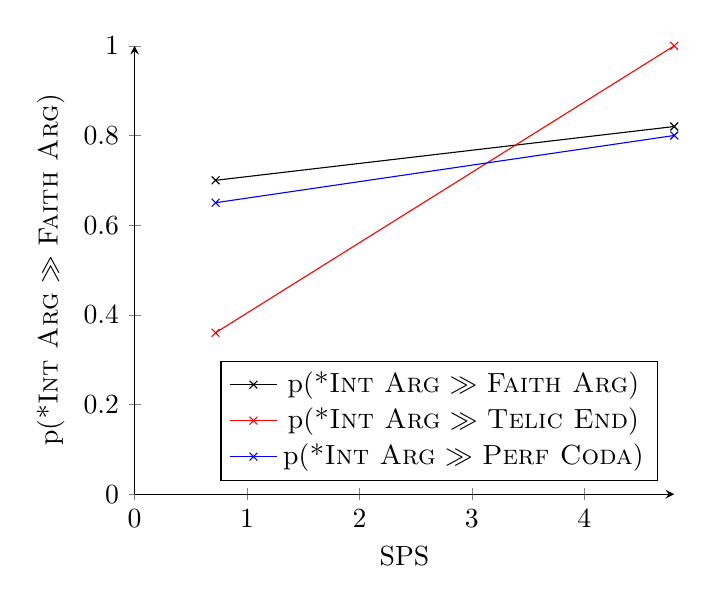
\begin{tikzpicture}
    \begin{axis}[legend pos=south east, xmin=0, ymin=0, ymax=1, axis lines = left,scaled ticks=false, xlabel={SPS}, ylabel={p(\textsc{*Int Arg} $\gg$ \textsc{Faith Arg})}] 
        \addplot[color=black,mark=x] coordinates {
        (0.72,0.70) 
        (4.80,0.82) 
    }; 
      \addlegendentry{p(\textsc{*Int Arg} $\gg$ \textsc{Faith Arg})};
            \addplot[color=red,mark=x] coordinates {
        (0.72,0.36) 
        (4.80,1.00) 
    }; 
    \addlegendentry{p(\textsc{*Int Arg} $\gg$ \textsc{Telic End})};
            \addplot[color=blue,mark=x] coordinates {
        (0.72,0.65) 
        (4.80,0.80) 
    }; 
    \addlegendentry{p(\textsc{*Int Arg} $\gg$ \textsc{Perf Coda})};
    \end{axis} 
\end{tikzpicture}
\end{figure}


\begin{figure}[htb]
\caption{Representation of the relationship between semantic selectivity and the probability of an implicit object output in Medina's model, based on computed $\gamma$ and $\delta$ values (reproduction of \reffig{medina_predictedresults}).}
\labfig{medina_predictedresults_new}
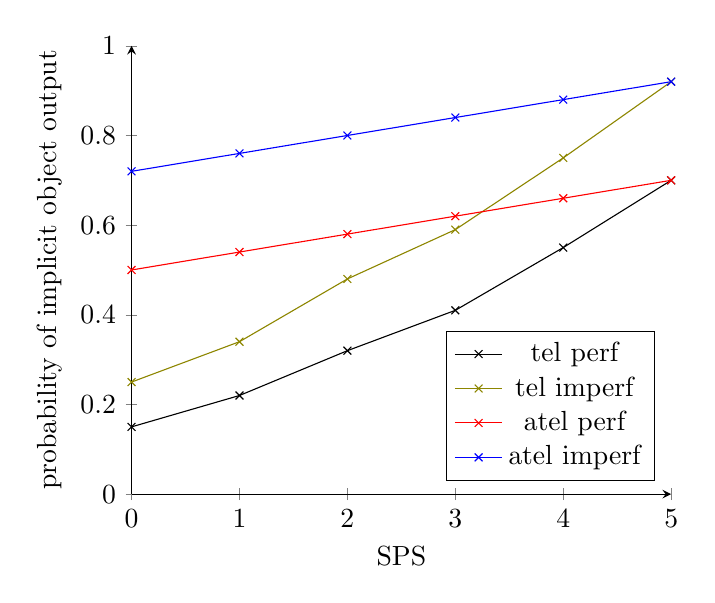
\begin{tikzpicture}
    \begin{axis}[legend pos=south east, xmin=0, ymin=0, ymax=1, axis lines = left,scaled ticks=false, xlabel={SPS}, ylabel={probability of implicit object output}] 
        \addplot[color=black,mark=x] coordinates {
        (0,0.15) 
        (1,0.22) 
        (2,0.32) 
        (3,0.41) 
        (4,0.55) 
        (5,0.70) 
    }; 
      \addlegendentry{tel perf};
        \addplot[color=olive,mark=x] coordinates {
        (0,0.25) 
        (1,0.34) 
        (2,0.48) 
        (3,0.59) 
        (4,0.75) 
        (5,0.92) 
    }; 
      \addlegendentry{tel imperf};  
        \addplot[color=red,mark=x] coordinates {
        (0,0.50) 
        (1,0.54) 
        (2,0.58) 
        (3,0.62) 
        (4,0.66) 
        (5,0.70) 
    }; 
      \addlegendentry{atel perf};    
        \addplot[color=blue,mark=x] coordinates {
        (0,0.72) 
        (1,0.76) 
        (2,0.80) 
        (3,0.84) 
        (4,0.88) 
        (5,0.92) 
    }; 
      \addlegendentry{atel imperf};        
    \end{axis} 
\end{tikzpicture}
\end{figure}

The same results I obtained in my basic model with semantic selectivity computed via Resnik's SPS are reported here in \reffig{eng_basic_sps_alltogether} and \reffig{eng_basic_sps_aspectualtypes}.


\begin{figure}[htb]
\caption{Probability of \textsc{*Int Arg} being ranked above each of the other constraints, varying in accordance with Behavioral PISA (English full model).}
\labfig{eng_basic_sps_alltogether}
    \input figures/eng_basic_sps_prob_alltogether.tex
\end{figure}

\begin{figure}[htb]
\caption{Probability of an implicit object output for each aspectual type, as a function of Behavioral PISA (English full model).}
\labfig{eng_basic_sps_aspectualtypes}
    \input figures/eng_basic_sps_prob_aspectualtypes.tex
\end{figure}

As is made evident by comparing \reffig{medina_intargabove_new} and \reffig{eng_basic_sps_alltogether}, my SPS-based basic model fails to reproduce Medina's findings. In Medina's model there is a prominent interaction between the probability of \textsc{*Int Arg} outranking \textsc{Telic End} and the probability of it outranking the two other constraints at play (i.e., \textsc{Faith Arg} and \textsc{Perf Coda}), while this interaction is absent from my SPS-based model. In particular, the relative re-ranking probabilities are ordered the same way in both models when Resnik's SPS (raw in Medina's plot, normalized in mine) is very low, i.e., \textsc{*Int Arg} is most likely to outrank \textsc{Faith Arg}, then \textsc{Perf Coda}, then \textsc{Telic End}. However, while in my model this relation also holds for high values of SPS, in Medina's model \textsc{*Int Arg} becomes more likely to outrank \textsc{Telic End} than other constraints for mid-to-high values of SPS.\\
This state of affairs is reflected in the probability of licensing an implicit object output for each separate aspectual type, reported here in \reffig{eng_basic_sps_alltogether} for Medina's model and in \reffig{eng_basic_sps_aspectualtypes} for my SPS-based basic model. Indeed, while in both models the object-dropping probabilities for the four aspectual inputs are ordered the same way for low-SPS verbs (atelic imperfective $\gg$ atelic perfective $\gg$ telic imperfective $\gg$ telic perfective), in Medina's model telic imperfective inputs are actually more likely to drop their object than atelic perfective inputs for mid-to-high-SPS verbs. In my model these probabilities vary according to SPS, but they never interact with one another.\\
However, it is interesting to note that I reproduced Medina's findings in my basic model using Computational PISA and, a bit worse, in my basic model using Behavioral PISA. I will not report here the four figures to avoid cluttering these pages, but the interested reader can compare Medina's figures with my own ones relative to the Computational PISA model (\reffig{eng_models_basic_cpisa_alltogether} and \reffig{eng_models_basic_cpisa_aspectualtypes}) and to the Behavioral PISA model (\reffig{eng_models_basic_bpisa_alltogether} and \reffig{eng_models_basic_bpisa_aspectualtypes}), collected in \refapp{app_models}. Since Medina considered a different set of verb than I did, and recruited 15 different participants than the 30 ones who participated in my experiment, it is possible to conclude that the grammar of English with respect to object drop defined by Medina is indeed true to the way native speakers of English re-rank the constraints to judge the grammaticality of object drop in their language. Crucially, Medina's results are not an artifact of the specific verbs she picked (the same as in \textcite{Resnik1993, Resnik1996}, for evident computational reasons). Why are her findings reproduced quite closely by my PISA-based basic models but not by my SPS-based basic model, which after all uses the very same measure of semantic selectivity Medina used? I would motivate these results by making reference to the shortcomings of Resnik's SPS, which I discussed extensively in \refsec{predictor_sps}, and in particular to its need for both a taxonomy (such as WordNet) and for a corpus (to extract the frequencies needed in the computation, as in \refsec{resnik_sps}). It is thus unsurprising that a model making use of a taxonomy-based measure yields results of fleeting reproducibility, even more so considering that the corpus upon which Resnik and Medina based their calculations (the Brown corpus) is much smaller than the one I employed to obtain Computational PISA scores (the ukWaC corpus).


\subsection{On regression models} \labsec{concl_lmem}

I would finally like to echo \posscite{Medina2007} concerns about the possibility of using a statistical regression model as a linguistically-informed model of language. In her thesis \parencite[132-133]{Medina2007}, she concluded that her Stochastic Optimality Theoretic model shares the property of additivity with linear regression models, since the former models the probability of an implicit object output as the sum of the probabilities of the relevant constraint re-rankings, while the latter models it as the sum of weighted variables. The main difference between the two kinds of model lies in the fact that the linguistic model keeps the input, the constraints, and the constraint re-rankings explicit, while in a regression model they are collapsed into weighted variables. In general, \textcite{PaterEtAl2006} observe that harmonic grammars\sidenote{That is to say, grammars selecting the most harmonic output among the candidates generated on the basis of the input, where "harmony" is the satisfaction of a set of weighted constraints. Refer to \refch{modeltheory} for more details.} translate into linear systems of equations and, thus, are solvable as such.\\
I second Medina's conclusions, based on the results I obtained in my own study (refer back to \refch{results} for the linear regressions and to the current Chapter for the linguistic models). In particular, I am going to compare the linear mixed-effects model\sidenote{Which, I will remember, is simply a linear regression model taking both fixed and random effects into account.} in \reftab{eng_lmem_bpisa} for English and in \reftab{ita_lmem_bpisa} for Italian with the results of my full linguistic model of object drop in \reffig{eng_ext2_bpisa_aspectualtypes} for English and in \reffig{ita_ext2_bpisa_aspectualtypes} for Italian. The mixed models clearly capture the main aspects of the linguistic models, e.g., the prominent role of telicity and perfectivity in jointly determining the grammaticality of the implicit object construction and the statistically less relevant effect of manner specification and iterativity. The role of Behavioral PISA determines another major divide between the two kinds of model, since in the regression it is assigned a weight just like any other predictor, be it continuous or binary, while in the Stochastic Optimality Theoretic model it is used as the independent variable in the computation of separate re-ranking functions for each constraint at play.\\
It is worth noting that Medina's model makes explicit use of a tenet of regression models, i.e., the requirement for the model to minimize the Summed Squared Error, which the reader can find in Medina's formulation on \refpage{medinaexcelsolver} (and again in \refsec{stot_full_fitting}) and in a more mathematically intense fashion in \textcite[13]{r_lmer} with regards to linear mixed-effects models. In a sense, a theoretical and computational method bridging the gap between linear regressions, which are linguistically naive, and Medina's model, which is not thoroughly defined as a linguistically-informed regression model, is Linear Optimality Theory \parencite{Keller2000, Keller2006}, a stochastic variant of Optimality Theory which represents the constraint rankings as numerical weights and has the grammaticality of any linguistic structure be proportional to the sum of the weights of the constraints it violates. While both Keller's Linear Optimality Theory and Medina's variant of Stochastic Optimality Theory rely on the Least Square Estimation algorithm to estimate parameters, the two models differ significantly in their implementation because Linear Optimality Theory defines grammaticality in terms of the relative harmony of two candidates in the same candidate set, while Medina's model evaluates the grammaticality of null-object candidates across candidate sets (for reasons explained in \refsec{ot_bad_dobjdrop}).
